% --------------------------------------------------------------------------- %
% Author:          Joey Dumont                <joey.dumont@gmail.com>         %
% Date created:    Mar. 8th, 2017                                             %
% Description:     Ph. D. thesis file.                                        %
% License:         CC0                                                        %
%                  <https://creativecommons.org/publicdomain/zero/1.0>        %
% --------------------------------------------------------------------------- %

% --------------------------------------------------------------------------- %
% --                               Preamble                                -- %
% --------------------------------------------------------------------------- %

% ----------------------------------------------------------------- %
% --                       Document Class                        -- %
% ----------------------------------------------------------------- %

\PassOptionsToPackage{table}{xcolor}
\documentclass[11pt,SymmetricalJury]{inrsthesis/inrsthesis}
\usepackage{lipsum}
% ----------------------------------------------------------------- %
% --                          Packages                           -- %
% ----------------------------------------------------------------- %



% -- Math symbols and fonts.
\let\mathfrak\undefined
\usepackage[charter]{mathdesign}      % Bitstream Charter for best font.
\usepackage[no-math]{fontspec}
\setmainfont{EB Garamond}
\usepackage[varg]{newtxmath}
% \usepackage{unicode-math}

\usepackage{microtype}   % Fine small typographical details
\usepackage{realscripts} % Use the font's sub- and superscripts
\usepackage{multirow}
\usepackage{dcolumn}

% %\usepackage[scaled=.96]{XCharter}
% \setmainfont{XCharter}
% \setmathfont{XCharter}

% Style and PDF formatting options.
%\usepackage[compact,sf]{titlesec}     % Use sans serif fonts in section headings.
\usepackage[bottom,
            multiple,
            stable]
           {footmisc}                % Force les notes de bas de page à être en bas de la page.

\usepackage[switch,mathlines,displaymath]{lineno}
\newcommand*\patchAmsMathEnvironmentForLineno[1]{%
 \expandafter\let\csname old#1\expandafter\endcsname\csname #1\endcsname
 \expandafter\let\csname oldend#1\expandafter\endcsname\csname end#1\endcsname
 \renewenvironment{#1}%
    {\linenomath\csname old#1\endcsname}%
    {\csname oldend#1\endcsname\endlinenomath}}%
\newcommand*\patchBothAmsMathEnvironmentsForLineno[1]{%
 \patchAmsMathEnvironmentForLineno{#1}%
 \patchAmsMathEnvironmentForLineno{#1*}}%
\AtBeginDocument{%
\patchBothAmsMathEnvironmentsForLineno{equation}%
\patchBothAmsMathEnvironmentsForLineno{align}%
\patchBothAmsMathEnvironmentsForLineno{flalign}%
\patchBothAmsMathEnvironmentsForLineno{alignat}%
\patchBothAmsMathEnvironmentsForLineno{gather}%
\patchBothAmsMathEnvironmentsForLineno{multline}%
}
\linenumbers
\usepackage[showframe,pass]{geometry} % Shows the frame properly when using memoir.
\usepackage[theorems=false]{latex-tools/vphys}        % Common LaTeX tools that I use.
\usepackage{latex-tools/celldraw}
\usepackage{todonotes}
\usepackage{booktabs}
\usepackage{siunitx}
\usepackage{subcaption}
\let\newfloat\undefined
\usepackage{floatrow}


\usepackage[unicode=true,
      pdfauthor={Joey Dumont},
      pdftitle={},
      bookmarks=true,
      bookmarksnumbered=true,
      bookmarksopen=true,
      bookmarksopenlevel=3,
      breaklinks=false,
      pdfborder={0 0 0},
      backref=false,
      colorlinks=true,
      linktoc=page,
      linkcolor=red,
      citecolor=blue,
      urlcolor=blue]
           {hyperref}

\usepackage[numbers,square,sort&compress]{natbib}
\usepackage{grffile}
\usepackage{calc}

% ----------------------------------------------------------------- %
% --                        Customization                        -- %
% ----------------------------------------------------------------- %
\newenvironment{chaptersummary}{%
  \begin{quotation}
  \SingleSpacing
  \setlength{\parskip}{\baselineskip}}{%
  \end{quotation}}

\allowdisplaybreaks

\settocdepth{section}
\setsecnumdepth{subsection}

%\captionsetup[figure]{labelfont=bf,width=0.85\textwidth}
%\captionsetup[table]{labelfont=bf,width=0.85\textwidth}


% Configuration of subcaptions.
\renewcommand\thesubfigure{\alph{subfigure}}
\renewcommand\thesubtable{\alph{subtable}}
  \captionsetup[figure]{width=0.90\textwidth,labelfont={sf,bf},textfont=sf,font+=small}
  \captionsetup[subfigure]{width=0.8\linewidth,parskip=0pt,font+=small}
  \captionsetup[table]{width=0.90\textwidth,labelfont={sf,bf},textfont=sf,font+=small}
  \captionsetup[subtable]{width=\linewidth,parskip=0pt,font+=small}

\usetikzlibrary{tikzmark,calc}

% ----------------------------------------------------------------- %
% --                       Title Page Info                       -- %
% ----------------------------------------------------------------- %
\title{Strong-field quantum electrodynamics \\ in tightly focused fields}
%\subtitle{Towards a Realitnatbibic Modelling of High-Power \\Laser Systems in the Quantum Theory}
\author{Joey Dumont}
\year{2018}
\program{Sciences de l'énergie et des matériaux}
\centreINRS{Centre Énergie Matériaux et Télécommunications}
\jury{
  \juryitem
    {Président du jury et \\ examinateur interne}
    {Nom du professeur \\ Institution}
  \\
  \juryitem
    {Examinateur externe}
    {Nom du professeur \\ Faculté ou département \\ Institution}
  \\
  \juryitem
    {Examinateur interne}
    {Nom du professeur \\ Institution}
  \\
  \juryitem
    {Directeur de recherche}
    {Jean-Claude Kieffer \\ INRS-ÉMT}
  \\
  \juryitem
    {Codirecteur de recherche}
    {Steve MacLean \\ INRS-ÉMT \\ University of Waterloo}
}
% --------------------------------------------------------------------------- %
% --                               Document                                -- %
% --------------------------------------------------------------------------- %

\begin{document}

\frontmatter

\maketitle

\chapter{Résumé}

Mots-clés:

\chapter{Abstract}

Keywords:

\chapter{Sommaire récapitulatif}
\cleardoublepage

\tableofcontents
\cleardoublepage

\listoftables
\cleardoublepage

\listoffigures
\cleardoublepage

\dedication{To my wife and son.}
\cleardoublepage

\epigraph{Whatever you do, do the best you can. The film lives forever!}{Jackie Chan}

\begin{flushright}
\begin{minipage}{0.35\textwidth}
The author claims that this statement not only applies for films with badass
action sequences, but for every artistic, cultural or scientific endeavour.
\end{minipage}
\end{flushright}

\cleardoublepage

\mainmatter

\chapter{Introduction}

\begin{chaptersummary}
  In this chapter, we place the contributions of this thesis in the context
  of the high-power laser literature and introduces some of the theoretical
  considerations on which this thesis will focus. We first discuss some recent
  advances in the development of high-power laser sources and their effect
  on the design of experimented aimed at measuring quantum electrodynamical
  effects in the strong field regime. The specific goals of this thesis are
  enumerated in \S\ref{sec:intro.objectives}.
\end{chaptersummary}

Quantum electrodynamics (QED) has been called the ``jewel of physics'' by one
of its most well-known contributor, Richard Feynman. Along with quantum
chromodynamics and electro-weak theory, which describe the strong and
weak nuclear force, respectively, QED describes the force that is closer
to our everyday life: electromagnetism\footnote{Even though it must be
said that classical electromagnetism should suffice in most
familiar situations.}.

Precision tests of QED.

\begin{figure}
  \centering
  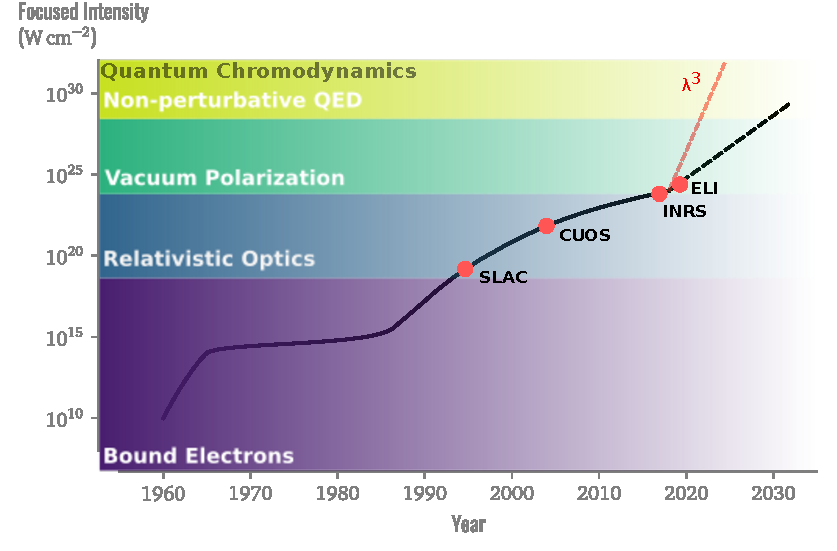
\includegraphics[width=0.9\textwidth]{figs/IntensityHistory.pdf}
  \caption[Short history of the intensity of laser systems.]
          {Intensity of laser systems as a function of time (approximative).
           Note that CPA has played a big role in accelerating the development
           of HPLs.
           Figured adapted from \cite{Mourou2015}.}
  \label{fig:intro.intensity-history}
\end{figure}

The advent of the chirped pulse amplification technique (CPA) has catapulted
the available focused laser intensities in the last three decades
\cite{Mourou2006}. Indeed, this technique has allowed an increase of about
6 orders of magnitude in the highest recorded intensity in a very short time
(Fig.~\ref{fig:intro.intensity-history}). This has opened up the possibility
of testing QED in a completely new sector of parameters.

The observation of strong-field quantum electrodynamics (SF-QED) processes with light
is contingent, for the most part, on the development of high-intensity laser sources \cite{DiPiazza2012}.
Reaching higher intensities can be achieved by (1) increasing the pump energy,
(2) shortening the pulse duration or (3) concentrating the beam in a small volume of space.
While recent laser systems have made significant advances on the first two items, there seems
to be technological difficulties in engineering gratings resistant enough to withstand the extreme
energy of the laser pulse.

\todo[inline]{Add more background on OPA laser systems. Paraxial propagation for most
  of laser chain, then non-paraxial effects in the last part of chain, just before
  the interaction region. Add figure. Check Mourou's review for technological issues
  related to HPLs.}

A promising avenue is the focusing of light down to extremely small volumes, on the order
of the wavelength of the radiation. In this regime, however, the oft used paraxial approximation
does not hold. This approximation is related to a Taylor expansion in terms
of the Lax parameter $\epsilon=\lambda/\pi w_0$ \cite{Lax1975}. In tightly focused
fields, $w_0\sim\lambda$ and the series does not converge \cite{Borghi2003}.

To see this, simply compare the fields of a ``focused'' paraxial beam with that
of a fully numerical solution of Maxwell's equations (more on that later).
\todo[inline]{Add figures of the fields separately, then show the overlap integral
  for each. Comment on it.}
Even with added terms, \ldots\todo[inline]{Same thing again.}
\todo[inline]{Applications in QED and other stuff to tightly focused fields.}

There also exists analytical solutions of Maxwell's equations that do not rely
on the paraxial approximation, such as e-dipole pulses and other models
\cite{Gonoskov2012,Salamin2015a,Salamin2015b}. They can be incredibly useful when used as part of
numerically-heavy codes, such as particle-in-cell codes because of their low
cost of evaluation. However, as any solution of Maxwell's equations in vacuum,
they do not take into account the minutiae of a given experimental setup
and thus fail to reproduce some details of tightly focused fields.
\todo[inline]{Argue why this is important.}

Although the availability of high-power lasers ($I\leq10^{22}\si{\watt\per\cm\squared}$)
is relatively recent, the study of quantum electrodynamics processes in the presence
of strong fields, a technical term to be defined a little later in this introcution,
dates back to the tail end of the 1920s. Klein's 1929's publication \cite{Klein1929} on a paradox
that now bears his name paved the way to the modelization of relatistivic
quantum effects. Sauter, in his 1931 paper \cite{SAU1931}, showed that the scale at which
these non-linear effects become important is given by what is now called
the Schwinger field,
  \begin{equation}
    E_S = \frac{m_e^2c^3}{e\hbar} \approx 1.3\times10^{18}\si{\volt\per\meter},
  \end{equation}
or rather the parameter
  \begin{equation}
    \eta = \frac{E_0}{E_S}
  \end{equation}
where $E_0$ is the amplitude of the background laser field. When $\eta\sim1$
in a static field,
it is expected that the dynamics are dominated by the breakdown of vacuum
into electron-positron pairs, until the depletion of the laser energy.
However, even future planned laser facilities will fall short of attaining
this extremely high electric field. Indeed, the Schwinger field corresponds
to an intensity of
  \begin{equation}
    I_S = \frac{1}{2}c\epsilon_0E_S^2\sim 2.24\times10^{29}\si{\watt\per\cm\squared},
  \end{equation}
and most planned facilities, such the European Extreme Light Infrastructure (ELI),
the French APOLLON, the Russian XCELS, the South Korean CoReLS, and (others)
do not plan on exceeding $10^{25}\si{\watt\per\cm\squared}$ (Fig.~\ref{fig:intro.intensity-history}).

HPL as another sector of QED to test. Complementary sector. New theoretical tools
needed (SF-QED). Insight into traditional QED as well?



\begin{figure}
  \centering
  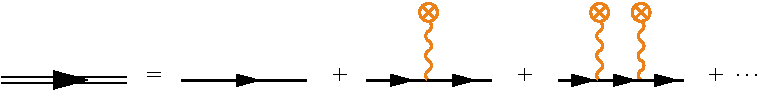
\includegraphics{figs/ResummedPropagator.pdf}
  \caption[Resummation of multiphotonic effects on the fermion propagator.]
          {When the multilphotonic parameter $\xi\geq1$, all these Feynman
          diagrams contribute to the same order. It is thus necessary to
          resum their contributions exactly, i.e. take into account
          the non-perturbative character of the interaction between the
          fermion and the laser field.}
  \label{fig:intro.resummed-propagator}
\end{figure}

When real electrons are involved in the process, the additional degrees of freedom
allow for the definition of new dimensionless parameters which govern the dynamics.
The first is similar to the Keldysh defined in the theory of ionization, as it
dictates whether multiphotonic are important. It is defined by
  \begin{equation}
    \xi = \frac{|e|E_0}{m_e\omega c}.
  \end{equation}
At low $\xi$, the probability that an electron interacts with $n$ photons
during its propagation scales as $P_n\sim\xi^{2n}$. In this regime,
only a few photons are exchanged between the laser and the electrons, and a
perturbative treatment makes. However, when $\xi\sim1$, multiphotonic effects
dominate and we must take into account the effect of the laser exactly.
In other words, it is necessary to exactly resum the $n$ photon interactions,
a procedure shown schematically in terms of Feynman diagrams in Fig.~\ref{fig:intro.resummed-propagator}.

The other important parameter is the laser field that the electron experiences
in its rest frame. It is simply given by
  \begin{equation}
    \chi = \frac{|e|\hbar\sqrt{\left(F^{\mu\nu}p_\nu\right)^2}}{c^3m_e^3} = \frac{(pk)}{(m_e c\omega)}\frac{E_0}{E_S}
  \end{equation}
where the second quality is valid in a plane wave.

Electron dynamics: introduction of xi and chi. xi >> 1 multiphotonic effects,
chi << 1, classical trajectories (no recoil).

SLAC E144, (multiple proposals since then, Karbstein et al), possible
detection of radiation reaction, proposals at ELI and other HPL facilities.



\begin{figure}
  \centering
  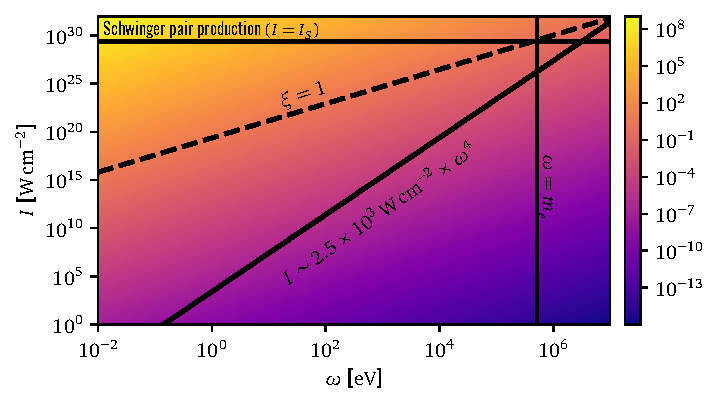
\includegraphics{figs/ClassicalLimit.pdf}
  \caption[Map of non-linearity parameters in intensity-frequency space.]
          {Value of the $\xi$ parameter as a function of intensity in \si{\watt\per\cm\squared}
          as a function of the frequency of the laser in \si{\eV}.}
  \label{fig:intro.xi-map}
\end{figure}

\section{Objectives and organization of this thesis}
\label{sec:intro.objectives}

The objectives of this thesis are to provide a flexible numerical tool that
can model the reflection of ultrashort pulses of arbitrary polarization, having
arbitrary temporal and spatial dependence off perfect conductors of complicated
geometry. Once that is done, we look for experimental configurations that either
optimize the yield of specific SF-QED observables, namely FWM \textit{in vacuo}
and Schwinger pair production. Using classical electron dynamics simulations, we
also wish to approximate the noise coming from competing processes in a low
density environment.

\begin{description}
  \item [Chapter \ref{chapter:stratton-chu} -- Tool 1: The Stratton-Chu Diffraction Integrals]
  test
  \item [Chapter \ref{chapter:fwm} -- ]
  test
  \item [Chapter \ref{chapter:electron_trajectories} -- ]
  test
\end{description}


% Basic plan:
%   \begin{itemize}
%     \item Generic introduction to SF-QED, experiments by SLAC and the upcoming
%           high power-laser facilities.
%     \item Motivation to accurately model the tight focusing regime: field inhomogeneities
%           play an important role in the detection of SF-QED observables (cite recent work by Di Piazza).
%     \item Approach based on two steps: modelling the optical side of things, then the quantum side of things.
%     \item Motivation behind the StrattoCalculator (vs Richards-Wolf, vs analytical solutions).
%     \item Mention going with focal point inside parabola.
%     \item Motivation behind SK (vs effective methods, vs analytical solutions). BONUS: inclusive observables.
%     \item Discussion of the use of HPC resources as a driver of future SF-QED experiments?
%   \end{itemize}

% Stuff to put in appendices:
%   \begin{enumerate}
%     \item Details of the Stratton-Chu formalism, perhaps some stuff on
%           discontinuity ``problem'' \cite{Asvestas1980} and the heuristic argument as to why
%           the physical approximation is correct.
%     \item Expressions of identity operators in Fock space for photons and fermions.
%     \item Proof that disconnected vacuum diagrams vanish identically in the SK formalism.
%     \item Minor results related to the \texttt{StrattoCalculator}:
%       \begin{itemize}
%         \item Gouy phase and its transverse momentum interpretation.
%         \item Work on the generation of pseudo-radially polarized beams with mosaics of half-wave plates?
%       \end{itemize}
%   \end{enumerate}

\chapter{Eletromagnetic Fields in the Tight Focusing Regime: The Stratton-Chu Diffraction Integrals}
\label{chapter:stratton-chu}

% \begin{chaptersummary}
%   This chapter discusses the problem of properly modelling electromagnetic fields
%   in the tight focusing regime. We first lay the foundation of electromagnetic
%   scattering and justify the choice of the Stratton-Chu formalism. Our numerical
%   implementation of this formalism is then discussed at length, and our results
%   are benchmarked against analytical results and results from the literature.
%   We briefly discuss the Richards-Wolf formalism, which is similar but not equivalent
%   to the Stratton-Chu formulation.
% \end{chaptersummary}

In this chapter, we introduce a fully numerical implementation of the Stratton-Chu
equations used to model the spatio-temporal focusing properties of large
bandwidth laser pulses focused by high numerical aperture optics. First, we
provide a detailed review of the Stratton-Chu integral representation and discuss
their reduction to a set of diffraction integrals. \todo{Finish division paragraph.}
It is then possible to write down an iterative solution to these integrals, the
first term of which is called the physical optics approximation. The resulting
quadrature is the basis of our model of tightly focused fields.

\section{Derivation of the Stratton-Chu Diffraction Integrals}

The derivation of the Stratton-Chu equations is fairly standard, and has been
written about many times \cite{}. Here, however, we follow Sancer's derivation,
whose exhaustive approach allows for a more thorough discussion.

The theoretical setup is as follows. Electric and magnetic currents\footnote{Magnetic
currents are used as a stand-in for an incident electric field \cite{Schelkunoff1936}.}
whose support are $V_e$ and $V_m$, respectively, are supposed to exist in free
space, denoted by $V_\infty$ (Fig.~\ref{fig:sc.scatteringSystem}). Later in the
derivation, integrals over these currents will be taken to represent the incident
field.

  \begin{figure}
    \centering
    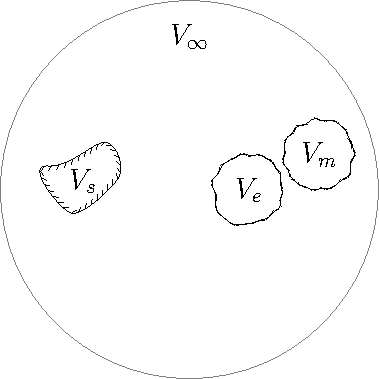
\includegraphics{figs/scatteringSystem.pdf}
    \caption[Geometry used in the derivation of the Stratton-Chu equations.]
            {Geometry used in the derivation of the Stratton-Chu equations.
             $V_s$ contains the scattering object, while $V_e$ and $V_m$ are the
             support of the electric and magnetic current distribution fonctions.
             $V_\infty$ represents free space, minus the scatterer, i.e.
             $V_\infty=\mathbb{R}^3\backslash V_s$.}
    \label{fig:sc.scatteringSystem}
  \end{figure}

The starting point is, as usual, the Maxwell equations. Their macroscopic version,
in Lorentz-Heaviside units with $c=1$, read
  \begin{subequations}
  \begin{align}
    \nabla\times\vb{E} + \frac{\partial\vb{B}}{\partial t}  &= \vb{J}_m \\
    \nabla\times\vb{H} - \frac{\partial\vb{D}}{\partial t}  &= \vb{J}_e
  \end{align}
  \end{subequations}
where $\vb{E}$ is the electric field, $\vb{B}$ is the magnetic field,
$\vb{D}$ the electric displacement, and $\vb{H}$ the magnetic field strength.
$\vb{J}_e$ is an electric current distribution that generates the incident
magnetic field and $\vb{J}_m$ is a fictitious magnetic current distribution
that generates an incident electric field. We will mostly be interested
in the electromagnetic field distribution in the $V_\infty$ region, i.e.
in vacuum. In this case, we have $\vb{D}=\vb{E}$ and $\vb{H}=\vb{B}$.

We first take the Fourier transform of the fields, i.e.
  \begin{equation}
    \mathcal{F}\left\{\vb{A}(\vb{r},t)\right\}(\vb{r},\omega)
                      = \int_{-\infty}^\infty \vb{A}(\vb{r},t)e^{-i\omega t }dt
  \end{equation}
and then take the curl of both equations.\todo[inline]{How much of the derivation do I
  actually want to show? Some key aspects to show off the discontinuity
problem should be enough, probably.}

Finally, we can derive this representation for the electromagnetic field,
in Fourier space,
  \begin{subequations}
  \label{eq:sc.field-stratton-chu-sancer}
  \begin{align}
  \vb{E}' &=
     \vb{E}_\text{inc}'+\iint_{S}
    \left\{ ik(\vu{n}\times \vb{B})              g
          +   (\vu{n}\times \vb{E})\times \nabla g
          +\frac{i}{k}\nabla\nabla g\cdot(\vu{n}\times\vb{B})
    \right\} dS,
  \label{eq:sc.efield-stratton-chu-sancer}\\
  \vb{B}' &=
    \vb{B}_\text{inc}' + \iint_{S}
    \left\{-ik(\vu{n}\times \vb{E})              g
          +   (\vu{n}\times \vb{B})\times \nabla g
          -\frac{i}{k}\nabla\nabla g\cdot(\vu{n}\times\vb{E})
    \right\} dS.
  \label{eq:sc.bfield-stratton-chu-sancer}
  \end{align}
  \end{subequations}
valid $\forall\vb{r}'\in V_\infty$. In these equations, $\{\vb{E}_\text{inc},\vb{B}_\text{inc}\}$
are the incident fields and are assumed
to arise from the sources and currents in $V_e$ and $V_m$, respectively.The primed coordinates
represent any point in $V_\infty$, while the unprimed coordinates represent points
on $S$, and are integrated over. $\{\vb{E}', \vb{B}'\}$ thus represent the field at any
given point in $V_\infty$, while $\{\vb{E}, \vb{B}\}$ denote the field on the surface $S$.
The notation $\vb{E}'$ [$\vb{E}$] is short for $\vb{E}(\vb{r}',k)$ [$\vb{E}(\vb{r},k)$]
where $k=2\pi/\lambda$ is the wavenumber of the laser pulse. $g$ is the scalar Green's function
  \begin{equation}
    g(\vb{r},\vb{r}') = \frac{e^{ik|\vb{r}-\vb{r}'|}}{4\pi|\vb{r}-\vb{r}'|}.
  \end{equation}
It is the only factor in Eq.~\eqref{eq:sc.field-stratton-chu-sancer}
that depends on both the integration variables $\vb{r}$
and the observation variables $\vb{r}'$.

Equation (\ref{eq:sc.field-stratton-chu-sancer}) is an integral representation
that expresses the field at any point in $V_\infty$ as integrals of the (yet unknown)
fields $\{\vb{E},\vb{B}\}$ over the surface of the scatterer.
To find the value of the fields on the scatterer, we take the limit $\vb{r}'\rightarrow S$.
This results in an integral equation on $S$, which can be solved iteratively. However,
care must be taken in the evaluation of this limit as $g$ has a simple pole at $\vb{r}=\vb{r}'$,
i.e. on the surface of the mirror.
This singularity is dealt with analytically by deforming the surface at $\vb{r}=\vb{r}'$
to a hemispherical surface with vanishing radius $R$. Let this contour be $S_\epsilon$. The
surface integrals can now be written as
  \begin{align}
    \lim_{\vb{r}'\rightarrow S}\iint_S \left\{\cdot\right\} dS
        &= \lim_{R\rightarrow0}\left(\iint_{S/S_\epsilon}+\iint_{S_\epsilon}\right) \left\{\cdot\right\}dS,
  \end{align}
where $\{\cdot\}$ represents any function. Evaluating this limit for each term separately
yields (the details of the computation are left for Appendix~\ref{app.limits}):
  \begin{subequations}
  \label{eq:sc.singularLimits}
  \begin{align}
    \lim_{\vb{r}'\rightarrow S}\iint_S \vb{A}g dS &= \miint{\rule{1em}{0.5pt}}_S \vb{A}g dS\label{eq:sc.regularLimit}, \\
    \lim_{\vb{r}'\rightarrow S}\iint_S \vb{A}\times\nabla gdS &= \frac{1}{2}\vb{A}\times\vu{n} + \miint{\rule{1em}{0.5pt}} \vb{A}\times\nabla gdS,\label{eq:sc.singularLimit}\\
    \lim_{\vb{r}'\rightarrow S}\iint_S \nabla\nabla g\cdot\vb{A}dS &= \HadamardSurf_S \nabla\nabla g \cdot\vb{A} dS\label{eq:sc.hypersingularLimit},
  \end{align}
  \end{subequations}
where $\vb{A}=\vu{n}\times\vb{F}$ and $\vb{F}$ stands for either the electric or
magnetic field. Equations (\ref{eq:sc.regularLimit}-\ref{eq:sc.singularLimit})
use the Cauchy principal value, denoted by $\CauchySurf$, and Eq.~\eqref{eq:sc.hypersingularLimit}
the Hadamard finite part \cite[Eq. (2.5)]{Blanchet2000}, denoted by $\HadamardSurf$.
Substituting the results of Eq.~\eqref{eq:sc.singularLimits} in the limit
$\vb{r}'\rightarrow S$ of Eq.~\eqref{eq:sc.field-stratton-chu-sancer}
yields the hypersingular integral equations
  \begin{subequations}
  \label{eq:sc.field-stratton-chu-sancer-hypersingular}
  \begin{align}
  \label{eq:sc.efield-stratton-chu-sancer-hypersingular}
  \vb{E} &= \vb{E}_\text{inc}+ \frac{1}{2}(\vu{n}\times\vb{E})\times\vu{n}
          +\CauchySurf_S
            \left\{ ik(\vu{n}\times \vb{B})              g
                    +   (\vu{n}\times \vb{E})\times \nabla g\right\}dS
          +\HadamardSurf_S\frac{i}{k}\nabla\nabla g\cdot(\vu{n}\times\vb{B}) dS,\\
  \label{eq:sc.bfield-stratton-chu-sancer-hypersingular}
  \vb{B}
      &= \vb{B}_\text{inc} + \frac{1}{2}(\vu{n}\times\vb{B})\times\vu{n}
      +\CauchySurf_S
        \left\{-ik(\vu{n}\times \vb{E})g +(\vu{n}\times \vb{B})\times \nabla g\right\}dS
      -\HadamardSurf_S\frac{i}{k}\nabla\nabla g\cdot(\vu{n}\times\vb{E})dS,
  \end{align}
  \end{subequations}
for $\vb{r}\in S$. Note that there are no more primed coordinates, as the integral
equations (\ref{eq:sc.field-stratton-chu-sancer-hypersingular})
are valid only for points on the surface of the mirror.

Although it may seem surprising for the
physical electromagnetic fields to be represented by hypersingular integrals,
the singularity is actually caused by the physical discontinuity in the reflecting surface.
The hypersingularity in Eqs.~\eqref{eq:sc.field-stratton-chu-sancer-hypersingular}
disappears if the surface $S$ is closed. Applying Stokes' theorem to the double gradient
term in Eqs.~\eqref{eq:sc.field-stratton-chu-sancer} yields the usual Stratton-Chu
representation for the fields in $V_\infty$
  \begin{subequations}
  \label{eq:sc.field.stratton-chu}
  \begin{align}
    \vb{E}'   &= \vb{E}_\text{inc}'+\frac{1}{ik}\oint_{\partial S} \nabla g \vb{B}\cdot d\vb{\ell}
                  + \int_S\left\{ ik(\vu{n}\times\vb{B})g
                  + (\vu{n}\times\mathbf{E})\times\nabla g
                  + (\vu{n}\cdot\vb{E})\nabla g
                 \right\} dS, \\
    \vb{B}'   &= \vb{B}_\text{inc}'-\frac{1}{ik}\oint_{\partial S} \nabla g \vb{E}\cdot d\vb{\ell}
                  + \int_S\left\{ ik(\vu{n}\times\vb{E})g
                  + (\vu{n}\times\mathbf{B})\times\nabla g
                  + (\vu{n}\cdot\vb{B})\nabla g
                 \right\} dS.
  \end{align}
  \end{subequations}
Taking the limit $\vb{r}'\rightarrow S$ as before reveals that all terms diverge
at most as $1/R^2$. This divergence can be readily integrated using the Cauchy
principal value for the terms inside the surface integral as the integration
measure cancels the divergence. However, this is not true for the terms contained in the line integral,
as the integration measure, $R$, does not cancel the divergence and the integral
is thus hypersingular. It can be shown that, before we take the limit $\vb{r}'\rightarrow S$,
the line integral itself vanishes identically
for a closed surface \cite{Sancer1968}, thus removing the hypersingularity.

Let us now go back to Eq.~\eqref{eq:sc.field-stratton-chu-sancer-hypersingular} and
impose the appropriate boundary conditions for a perfectly
conducting mirror \cite[Eq. (1.18)]{Stratton1941}, i.e.
  \begin{equation}
    \label{eq:sc.boundaryConditions}
    \vu{n}\times\vb{E}=0;\qquad \vu{n}\times\vb{B}=\vb{J}.
  \end{equation}
Extracting the tangential components of Eqs.~\eqref{eq:sc.field-stratton-chu-sancer-hypersingular}
and imposing these conditions yields
  \begin{subequations}
  \begin{align}
    -\vu{n}\times\vb{E}_\text{inc} &= \vu{n}\times\left[\CauchySurf_S ik\vb{J}g dS + \HadamardSurf_S\frac{i}{k}\nabla\nabla g\cdot\vb{J} dS\right],\\
    \label{eq:sc.mfie}
    \frac{1}{2}\vb{J}  &= \vb{J}_\text{inc} + \vu{n}\times\CauchySurf_S \vb{J}\times\nabla gdS,
  \end{align}
  \end{subequations}
where $\vb{J}_\text{inc}=\vu{n}\times\vb{B}_\text{inc}$.
Both equations can be solved for the current $\vb{J}$ induced by the incident
field $\{\vb{E}_\text{inc},\vb{B}_\text{inc}\}$. Since it can be shown that
the integral operator in the magnetic field integral equation, \eqref{eq:sc.mfie},
is compact, we can use the Liouville-Neumann series to solve the integral equation
iteratively \cite[\S6.16]{Jones1994}. The first term of the series yields the usual
physical optics approximation (POA)
  \begin{equation}
    \label{eq:sc.poa}
    \vb{J} = 2\vb{J}_\text{inc},
  \end{equation}
which coincides with the result for a plane, infinite mirror \cite[\S12.2]{Bladel2007}. The
integral in Eq.~\eqref{eq:sc.mfie} can thus be interpreted as a curvature effect.
Indeed, each term in the iterative solution can be shown to get gradually smaller
in magnitude if the radius of curvature is larger than the wavelength of the
incident radiation \cite{Cullen1958,Bladel2007}.
The POA has been used successfully in many studies \cite{Bouwkamp1954,Love1978}.

Substituting the POA [Eq.~\eqref{eq:sc.poa}] and the boundary conditions
[Eq.~\eqref{eq:sc.boundaryConditions}] in Eqs.~\eqref{eq:sc.field-stratton-chu-sancer},
we can express the reflected field $\vb{F}'_\text{ref}=\vb{F}'-\vb{F}_\text{inc}$
in $V_\infty$ as
  \begin{subequations}
  \label{eq:sc.stratton-chu-poa}
  \begin{align}
    \label{eq:sc.stratton-chu-poa.efield}
    \vb{E}'_\text{ref}  &=  2\iint_S
      \left\{
        ik(\vu{n}\times\vb{B}_\text{inc})g
        +\frac{i}{k}\nabla\nabla g\cdot(\vu{n}\times\vb{B}_\text{inc})
        \right\}dS, \\
    \label{eq:sc.stratton-chu-poa.bfield}
    \vb{B}'_\text{ref}  &= 2\iint_S (\vu{n}\times\vb{B}_\text{inc})\times\nabla g dS.
  \end{align}
  \end{subequations}
Even though Eqs.~\eqref{eq:sc.stratton-chu-poa} are valid expressions
for the reflected field, the double gradient term tends to strongly oscillate in applications and therefore
make its numerical evaluation difficult. We sidestep this issue by once again applying
Stokes' theorem on the double gradient term, which leads to
  \begin{subequations}
  \label{eq:sc.stratton-chu-poa-og}
  \begin{align}
    \label{eq:sc.stratton-chu-poa-og.efield}
    \vb{E}'_\text{ref}(\vb{r}',k)  &= 2\iint_S
      \left\{
        ik(\vu{n}\times\vb{B}_\text{inc})g
        +\left(\vu{n}\cdot\vb{E}_\text{inc}\right)\nabla g
        \right\}dS
            - \frac{2}{ik}\oint_{\partial S}\nabla g
                    \left[\vu{n}\times(\vu{n}\times\vb{B}_\text{inc})\right]\cdot d\vb{\ell},\\
    \label{eq:sc.stratton-chu-poa-og.bfield}
    \vb{B}'_\text{ref}(\vb{r}',k)  &= 2\iint_S (\vu{n}\times\vb{B}_\text{inc})\times\nabla g dS.
  \end{align}
  \end{subequations}
The double gradient term has been replaced by two terms: a surface term with a
single gradient and an additional line integral term  which also contains
a single gradient. The single gradient results in a $1/R$ behavior of the integrands,
compared to the $1/R^2$ of the double gradient. This weakens the oscillations of
the integrands.

Equations (\ref{eq:sc.stratton-chu-poa-og}) describe a spectral component
of frequency $k$ of the reflected field at a given position $\vb{r}'$ as an integral
of the incident field on the surface of the mirror. The remainder of this paper
will be devoted to their efficient numerical evaluation for arbitrary incident
fields $\{\vb{E}_\text{inc},\vb{B}_\text{inc}\}$ with complex time-dependence
and for arbitrary mirror geometries $S$.

\section{Practical Implementation}

The derivation above holds for a single component of the Fourier decomposition
of our assumed ultrashort pulse. To model the reflection of a short pulse, then,
it is necessary to repeat that calculation for each frequency component that
makes up the incident beam, and then to add them coherently.

Experimentally, we are usually given the energy of the pulse along
with its spectral characteristics. In the following paragraph, we will devise
a normalization scheme that allows us to model arbitrary incident beam models,
i.e. with arbitrary spatial and temporal dependence. Then, we will discuss
the details of the numerical evaluation of the integrals involved in the
Stratton-Chu formalism, more specifically the parallel domain decomposition
method used. We will also elaborate on an interesting property of paraboloid
mirrors: indeed, if the field is evaluated in a region close to the focal volume,
the Stratton-Chu integrands do not exhibit the highly oscillatory behaviour
typical of diffraction integrals.

In the last sections, we provide a detailed numerical verification of our
C++ implementation. This is crucial, as the author is not aware of any useful
analytical solutions to the Stratton-Chu equations that would allow an easy
verification of the implementation.


\subsection{Handling the Temporal Dynamics}

To properly model the temporal dynamics of the beam at focus, it is in principle
only necessary to know the temporal dynamics of the incident beam. However, in
an experimental setting, a complete temporal cartography of the field is usually
not readily available. Rather, the power spectrum and the (possibly spatially
dependent) spectral phase is available. To map these quantities to the input
of our Stratton-Chu equations, we will use the Poynting theorem to relate
the energy density of the pulse to the spatiotemporal characteristics of the
incident beam.

We assume that a quantity known as the spectral energy density (to be defined later),
the total energy, and the spectral phase are known. The total energy of the
beam can be computed via the Poynting theorem
  \begin{equation}
    E_\text{beam}
      =
      \int_{-\infty}^\infty \oiint_A
        \left[\vb{E}(\vb{r},t)\times\vb{B}(\vb{r},t)\right]\cdot d\vb{A}dt.
  \end{equation}
Substituting the Fourier transform of the fields, i.e.
  \begin{align}
    \vb{E}(\vb{r},t) &=
      \int_{-\infty}^\infty
        \vb{E}(\vb{r},\omega)e^{i\varphi(\omega)}e^{-i\omega t} d\omega \\
    \vb{B}(\vb{r},t) &=
      \int_{-\infty}^\infty
        \vb{B}(\vb{r},\omega)e^{i\varphi(\omega)}e^{-i\omega t} d\omega
  \end{align}
where $\varphi(\omega)$ is some phase that only depends on the frequency.
The total energy can then be written as
  \begin{equation}
    E_\text{beam} = 4\pi \oiint_A \int_0^\infty
        \real{\vb{E}(\vb{r},\omega)\times\vb{B}(\vb{r},\omega)}\cdot d\vb{A}d\omega
  \end{equation}
From this we define the spectral energy density,
  \begin{equation}
    \epsilon(\omega)
      = 4\pi\oiint_A \real{\vb{E}(\vb{r},\omega)\times\vb{B}(\vb{r},\omega)}\cdot d\vb{A}
  \end{equation}
Now, due to the linearity of Maxwell's equations, we can multiply the field
by an arbitrary complex number and still be solutions of the differential
equations. We thus write
  \begin{equation}
    \vb{E}(\vb{r},\omega) = E_0\vb{f}_E(\vb{r},\omega); \qquad
    \vb{B}(\vb{r},\omega) = E_0\vb{f}_B(\vb{r},\omega)
  \end{equation}
and rescale the fields according to
  \begin{equation}
    E_0 \mapsto \sqrt{%
      \frac{\epsilon_\text{exp}(\omega)}
           {4\pi\oiint_A\real{\vb{f}_E(\vb{r},\omega)\times\vb{f}_B(\vb{r},\omega)}\cdot d\vb{A}}
    }
    \label{eq:sc.normalization}
  \end{equation}
where $\epsilon_\text{exp}(\omega)$ is the experimentally known spectral density,
or power spectrum.

\todo[inline]{Add note on the fact that, experimentally, the spectral density
is actually integrated over a small frequency range? This fixes the units...}


\subsection{Spatial Discretization}

The Stratton-Chu equations (Eqs~\eqref{eq:sc.stratton-chu-poa-og}) reference two
separate spatial domains, the integration surface $S$ that the $\vb{r}$ variable
references, and the point at which the field is evaluated, $\vb{r}'$. There are
multiple advantages that stem form this: (1) the typical length scales of the
unfocused of the unfocused and focused fields can differ by orders of magnitude,
hence, their natural separation in the integral formulation makes their meshing
much easier, (2)  the field can be evaluated at any point of our choosing:
the method is not limited to a specific type of mesh.

In the implementation, we provide two modes of operation. Either we compute the
field at a user-specified point, or on a predefined mesh of points suitable
for integration for later use.

In the tight focusing regime, the electromagnetic field shows features that
are similar in size to the wavelength $\lambda$ of the radiation. Numerically,
then, the mesh size should be smaller than $\lambda$. However, the incident
beam usually has spatial variations on the order of the centimeter, orders
of magnitude larger than $\lambda$. In typical electromagnetic computational
methods, the limitation of a fixed size mesh throughout all space translates
in unrealistic memory requirements in the tight focusing regime. In the
Stratton-Chu formalism, the independence of the two domains makes it so
the meshes can be of different sizes.

However, to achieve sub-$\lambda$ resolution, memory requirements can still be
prohibitive for a single machine, typically a few gigabytes for each frequency
component. This is of course compounded by the fact that temporally short pulses
have broad spectra, requiring a large number of frequency components to properly
resolve. To mitigate this issue, it is thus necessary to perform the computations
on multiple machines simultaneously, in parallel.


\begin{figure}
%  \floatbox[{\capbeside\thisfloatsetup{capbesideposition={inside,top},capbesidewidth=4cm}}]{figure}[\FBwidth]
%{\caption{A test figure with its caption side by side}\label{fig:test}}
%{\includegraphics[width=5cm]{name}}
  \centering
  \floatbox[{\capbeside\thisfloatsetup{capbesideposition={right,center},capbesidewidth=0.3\textwidth}}]
  {figure}[\FBwidth]
  {\hspace{3cm}\captionsetup{width=0.4\textwidth}
  \caption[Domain decomposition strategy employed in the StrattoCalculator.]
          {Parallelization strategy used in the StrattoCalculator. The domain
          over which the integrals are evaluated is distributed among multiple
          processors, while the mesh over which the integrands are evaluated are
          global, i.e. they exist in each MPI process' region of memory.}
          \label{fig:sc.domain-decomposition}
  }
  {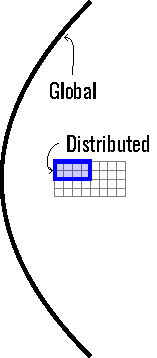
\includegraphics{figs/hpc-domaindecomposition.pdf}}
\end{figure}

Given that the field at a point $\vb{r}_1$ can be evaluated without any reference
to another point $\vb{r}_2$, the parallelization strategy is quite simply to
separate the focal volume into chunks with the same number of points and assign
these chunks to different processors (Fig.~\ref{fig:sc.domain-decomposition}).
Because the numerical cost of evaluating
the integral does not depend on the position at which the field is evaluated
(in our approach), the workload is thus evenly divided among the processors.

\subsubsection{Side note: phase cancellation in the paraboloid case}
\label{sec:sc.phase-cancellation}

Typically, diffraction integrals have an highly oscillatory behaviour that
stems from the propagator, or Green's function of the problem. The Stratton-Chu
integrals (or even the Richards-Wolf integrals, for that matter, although they
use a trick) are not exception. The diffraction integrals are of the generic form
  \begin{equation}
    I = \int f(\vb{r})e^{ikh(\vb{r},\vb{r}')}d\vb{r}
  \end{equation}
where $f(\vb{r})$ is a function of the incident fields and $h(\vb{r},\vb{r}'')$
is the phase function, typically the distance between the points $\vb{r}$ and
$\vb{r}'$, i.e. $h=|\vb{r}-\vb{r}'|$. In an optical setting, we expect this integrand to oscillate rapidly
as the wavelength of the radiation is much smaller than the size of the reflecting
mirror, i.e. $k|\vb{r}|\gg1$. Rapidly oscillating integrals of the form above
are difficult to evaluate numerically, although there are some techniques
that facilitate their evaluation in the case $k\rightarrow\infty$ \cite{Iserles2004,Ganesh2007}.

We show that, for a paraboloid mirror, a non-trivial cancellation in the phase function
results in the strength of the oscillations being dictated by the observation
variables $k|\vb{r}'|\simeq1$ rather than the integration variables $k|\vb{r}|\gg1$
(Fig.~\ref{fig:sc.oscillating-phase-with-distance}).
In this case, it is not necessary to use specialized techniques, nor to use
sub-$\lambda$ mesh resolution on the integration surface. In our implementation,
we use simple tensor products of either the Simpson or Gauss-Legendre methods
\cite[\S4.6]{Press1986}.

\begin{figure}
  \begin{subfigure}[t]{0.32\textwidth}
    \centering
    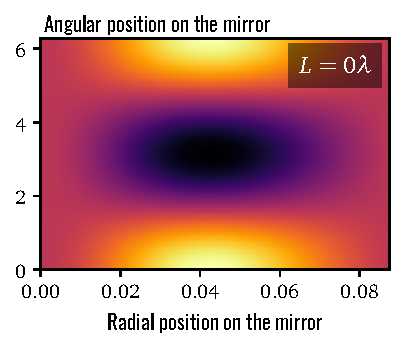
\includegraphics[width=\textwidth]{figs/phase_0L.pdf}
    \caption{Integrand for $E_r$ evaluated at the focal point.}
    \label{fig:sc.oscillating-phase-with-distance.0L}
  \end{subfigure}
  \hfill
  \begin{subfigure}[t]{0.32\textwidth}
    \centering
    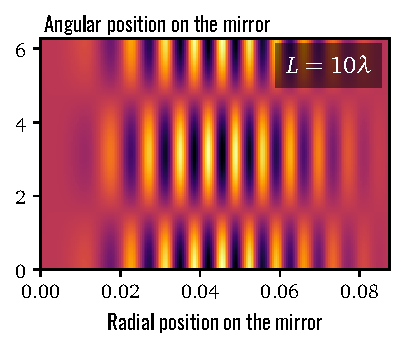
\includegraphics[width=\textwidth]{figs/phase_10L.pdf}
    \caption{Integrand for $E_r$ evaluated at a distance $10\lambda$ away from the focal plane.}
    \label{fig:oscillating-phase-with-distance.10L}
  \end{subfigure}
  \hfill
  \begin{subfigure}[t]{0.32\textwidth}
    \centering
    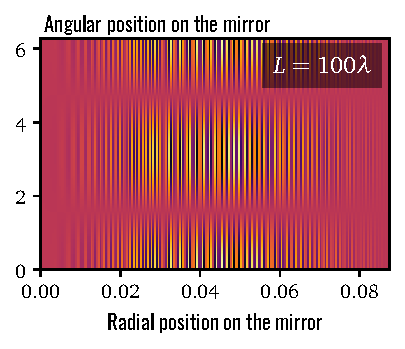
\includegraphics[width=\textwidth]{figs/phase_100L.pdf}
    \caption{Integrand for $E_r$ evaluated at a distance $100\lambda$ away from the focal plane.}
    \label{fig:oscillating-phase-with-distance.100L}
  \end{subfigure}
  \caption[Illustration of oscillation of the integrand with increasing distance from the focal point.]
          {Integrand of the $E_r$ component of a radially polarized beam with parameters given in
            Table \ref{tab:comparison.parameters}, for the frequency component at $\lambda=800\si{\nano\metre}$.
            \textbf{(a)} In the focal plane, the scale of the oscillations follows those of the incident
            Gaussian beam. As we increase the observation point further away from the focal point
            (see \textbf{(b)} and \textbf{(c)}), the strength of the oscillation increases in
            accordance with Eq.~\eqref{eq:sc.parabola-phase-taylor}.
          }
  \label{fig:sc.oscillating-phase-with-distance}
\end{figure}

The cancellation occurs when we consider the oscillatory behaviour of the
incoming field. In the paraxial approximation, the incoming field carries
a propagation phase such that $f(\vb{r})\propto e^{-ikz}$. Hence, the phase
function that determines the oscillatory behaviour is
$h(\vb{r},\vb{r}')=|\vb{r}-\vb{r}'|-z$. To determine whether the integrand
oscillate strongly, we examine this function in the vicinity of the focal
point, i.e. $\vb{r}'=0$ in our coordinates.
Expanding the phase function in a Taylor series, we have
  \begin{equation}
    h(\vb{r},\vb{r}') = \sqrt{r^2+z^2}-z
                  -\frac{r\cos(\theta-\theta')}{\sqrt{r^2+z^2}} r'
                  -\frac{z}{\sqrt{r^2+z^2}}z'
                  + \mathcal{O}\left[\left(\frac{r',z'}{|\vb{r}|}\right)^2\right]
  \end{equation}
Near the focal spot, then, the first-order terms oscillate slowly, because the prefactor
of each term has range $[-1,1]$ and $r'$ and $z'$
(the radial and longitudinal distances from the focal point)
do not exceed a few wavelengths, i.e. $k|\vb{r}'|\sim1$.
The zeroth-order term
is thus the only term that can lead to a rapidly oscillating
integrand.
For the specific of a parabolic mirror, for which $z=r^2/4f-f$, the phase function
reads
  \begin{equation}
    h(\vb{r},\vb{r}')\simeq 2f - \frac{4rf}{f^2+r^2} r' - \frac{r^2-4f^2}{r^2+4f^2} z' + \cdots
    \label{eq:sc.parabola-phase-taylor}
  \end{equation}
The zeroth-order term does not depend on the integration variables, implying
that the integrand does not oscillate at $\vb{r}'=0$ and oscillates weakly
in its vicinity.

This non-trivial cancellation does not carry over to generic surfaces, however.
For instance, the zeroth-order term does depend on the integration variables
in the ellipsoidal \footnote{More precisely,
mirrors of the form $z^2/c^2=1-(x^2+y^2)/a^2$, with focal spots
at $z=\pm\sqrt{c^2-a^2}$.} case. In fact, for other mirror geometries, the initial
physical motivation of looking at distances not too far away from the focal spot
might be lacking. For most mirrors, there are no uniquely
defined focal points and the field is diffuse. In these cases, care
should be taken when numerically evaluating the Stratton-Chu integrals.

\subsection{Incident Field Models}

Incident field models should try to replicate the experimental conditions
as close as possible. As the goal of the StrattoCalculator is to explore
and identify the most promising experimental designs, its free parameters
should be set as close as possible as those of the experiment. This limits
our set of approximations that we can use.

With that mind, we will use two main approximations. One, the incident field
is a solution of the paraxial wave equation. This is not a restricting approximation,
as the fields that modern laser systems output are highly collimated. Moreover,
the output through a hole restricts the waist of each of the frequency components
to be the same. In fact, most laser systems can be well-approximated by a
superposition of super-Gaussian beams, i.e. beams with the shape
  \begin{equation}
    f(r,\theta) \propto \exp\left[-\left(\frac{r}{w_0}\right)^{2n}\right]
  \end{equation}
where $n$ is the order of the super-Gaussian and $w_0$ is the beam waist.
$n=1$ refers to a standard Gaussian beam, of course.

While the Stratton-Chu equations do not explicitly require any assumption on
the incident field, it is useful to introduce some. In particular, we will be
interested in field models where the normalization constant [\eqref{eq:sc.normalization}]
can be computed analytically, as this can drastically reduce the setup time
of the computation. \todo{Why?}

Unfortunately, this precludes the direct use of the super-Gaussian function,
as it typically leads to non-integrable functions. Our strategy, then, will
be to use general solutions of the paraxial equation as a basis to express
arbitrary spatial dependence, including super-Gaussian dependence.


In vacuum, the electric field, magnetic field and vector potential all obey
the same differential equation, namely
  \begin{equation}
    \left(\nabla^2-\partial_t^2\right)\vb{F}(\vb{r},t) = 0
  \end{equation}
where $\vb{F}$ is any of the fields mentioned above. Solving this
in the Fourier domain and applying the paraxial approximation
yields
  \begin{equation}
    \left(\nabla_\perp^2-2ik\partial_z\right)\psi(r,\theta,z) = 0
  \end{equation}
where
  \begin{equation}
    \vb{F}(\vb{r},t) = \psi(r,\theta,z)e^{-i\omega t - ikz} \vu{z}.
  \end{equation}
The general solution reads \cite{Allen1992}
  \begin{multline}
    \psi(r,\theta,z) = \sum_{\ell=-\infty}^\infty\sum_{n=0}^\infty
      \frac{c_{n\ell}}{\sqrt{1+\left(\frac{z}{z_R}\right)^2}}
      \left(\frac{\sqrt{2}r}{w(z)}\right)
      L_p^\ell\left(\frac{2r^2}{w^2(z)}\right)\exp\left(-\frac{r^2}{w^2(z)}\right)
      \exp\left(-\frac{ikr^2}{2R(z)}\right)e^{-i\ell\theta}\\
      \times\exp\left[i\left(2n+\ell+1\right)\arctan\frac{z}{z_R}\right].
  \end{multline}

This equation can be used to describe both linearly and radially polarized
beams. Indeed, choosing $\vb{E}(\vb{r},t)=\psi(r,\theta,z)e^{-i\omega t -ikz}\vu{x}$,
we can describe a linearly polarized beam. Choosing $\vb{A}(\vb{r},t)=\psi(r,\theta,z)e^{-i\omega t - ikz}\vu{z}$
yields
  \begin{align}
    \vb{E}(\vb{r},k) &= ik\vb{A}+\frac{i}{k}\nabla\left(\nabla\cdot\vb{A}\right) \\
    \vb{B}(\vb{r},k) &= \nabla\times\vb{A}.
  \end{align}

\todo[inline]{This can be used as the basis to describe the Lax series
  that we discuss above. Maybe move this section?}

\todo[inline]{Add normalization in Appendix.}

\subsection{Parallelization and Performance Analysis}

When designing parallel applications, it is important to know how the implementation's
performance scales with the number of processors. Often, the most important
performance gains can be realized by changing the underlying algorithm that
is used to perform computations. When we are confident that the chosen algorithm
will provide the better scaling, it is useful to verify this scaling by measuring
the performance of the code as a function of the number of processors.

An important measure of scalability is the parallel efficiency, defined by the
formula
  \begin{equation}
    E_n = \frac{t_1}{nt_n}
  \end{equation}
where $E_n$ is the efficiency at $n$ processors and $t_m$ is the time for a typical
simulation run to execute on $m$ processors. Ideally, we would like
$E_n\equiv1\forall n$.

Of course, the performance increase is capped by Amdahl's law, which states that
the theoretical speedup of parallel program that is divided into a serial portion
$s$ and a parallel portion $p$ is given by
  \begin{equation}
    S = \frac{1}{1-p+\frac{p}{s}}
  \end{equation}
This can be misleading, as it is possible that other factors, such as a reduced
number of cache misses, occur when increasing the number of processors.
This could even lead to a parallel efficiency that is larger than 1.

The StrattoCalculator has two use cases: (1) we compute the field in the
focal spot and save it to a file for later analysis and (2) we compute the
field in the focal spot and use the field available in memory to compute
other observables. The former typically outputs large files, up to hundreds
of gigabytes in size. In turn, we expect its parallel efficiency to decrease
substantially, as the parallel I/O portion of the code will make up a larger
proportion of the runtime, and parallel I/O is very hard to scale. \todo{Citation.}
The latter is expected to scale perfectly, as the underlying algorithm is
embarrassingly parallel.

Running tests on two different clusters reveals that the parallel efficiency
greatly depends on the underlying hardware. In mp2, the test simulation
with data output does not scale well beyond 8 nodes, or 192 processors (Fig.~\ref{fig:sc.parallel-efficiency.mp2}.
On GP3, the implementation scales well, even at 1024 processors. We surmise that
the faster InfiniBand interconnects and a properly Lustre-optimized Parallel HDF5
module explains the much more efficient I/O, and therefore overall parallel efficiency
on GP3.

\begin{figure}
  \centering
  \begin{subfigure}[t]{0.47\textwidth}
    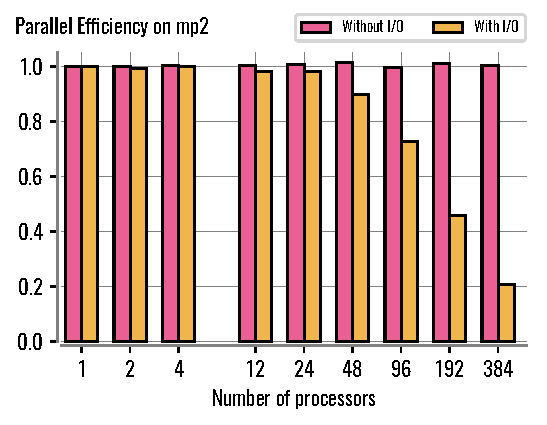
\includegraphics[width=\textwidth]{figs/ParallelEfficiency-mp2.pdf}
    \caption{Parallel efficiency of the StrattoCalculator on the mp2 Compute
             Canada cluster. 384 processors, or 16 nodes, is the maximum number
             of processors that can be requested on this cluster.}
    \label{fig:sc.parallel-efficiency.mp2}
  \end{subfigure}
  \hfill
  \begin{subfigure}[t]{0.47\textwidth}
    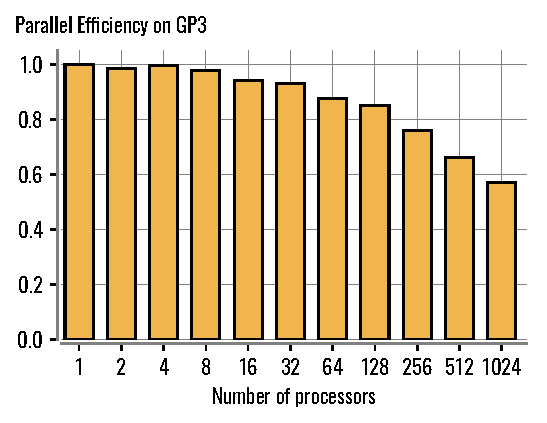
\includegraphics[width=\textwidth]{figs/ParallelEfficiency-gp3.pdf}
    \caption{Parallel efficiency of the StrattoCalculator on the GP3, also known
             as Graham, Compute Canada cluster. While 2048 is not the maximum number
             of processors we can ask for, the wait time would have been prohibitely
             long for a higher number of processors, given our low priority.}
    \label{fig:sc.parallel-efficiency.gp3}
  \end{subfigure}
  \caption{Parallel efficiency of the StrattoCalculator on different clusters.
           Notice that the efficiency is highly dependent on the cluster.}
  \label{fig:sc.parallel-efficiency}
\end{figure}

\section{Properties of Tightly Focused Fields}

In this section, we explore some properties of the fields in the focal
spot as a function of the focusing strength of the optics, i.e. the
focal length of the parabola.

Our main finding is that while the maximum intensity increase and the spot
size decreases with decreasing $\alpha=2f/r_\text{max}$, as expected, this behaviour
reverses when $\alpha$ goes below 1. We show that this can be explained by the
progressive increase in strength of the longitudinal components of the field, which
present two lobes in the focal plane, instead of the usual Gaussian dependence.
While this result is expected, what is more interesting is the effect this has
on SF-QED observables, to be discussed in the next chapter.

Typical optical setups use relatively long focal length parabolic mirrors
to transport the beam throughout the experiment chamber, and also
to focus it in some region of space where some experiment takes place.
A useful parameter that can be used to characterize the focusing of the parabola
is $\alpha=2f/r_\text{max}$, where $f$ is the focal length and $r_\text{max}$
is the radius of the aperture of the parabola. The usual parameter, the numerical
aperture, is defined geometrically as $NA=\sin\theta$, where $\theta$ is the
angle between the optical axis and the line that goes from the focal point
to the aperture. Our parameter has the advantage of being monotonic
in the focal length. Indeed, we will study configuration where the focal
point is \textit{inside} the paraboloid mirror, where the angle $\theta$
starts to decrease again. $\alpha$ is exactly 1 when the focal plane is aligned
with the aperture, smaller than one is the focal point is inside, and greater
than one if it is outside.

As mentioned in the introduction, the issue of bringing the focal plane
inside the parabola is that there exists rays that are reflected back into
the laser chain. These rays are extremely dangerous, as they could easily
destroy the laser system if they travel back down the chain. There are two
ways to solve this issue: (1) use a temporal gate to block the reflection
back into the chain (risky), or (2) remove the part of the parabola that
creates these backreflections.

\begin{figure}
  \begin{subfigure}[t]{0.47\textwidth}
    \centering
    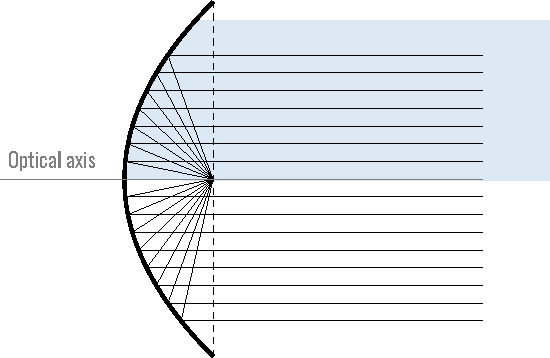
\includegraphics{figs/parabola_hna.pdf}
    \caption{Typical HNA parabola, where the focal plane either intersects or is
            farther away from the aperture plane of the parabola.}
    \label{fig:vsf-v-hna.hna}
  \end{subfigure}
  \hfill
  \begin{subfigure}[t]{0.47\textwidth}
    \centering
    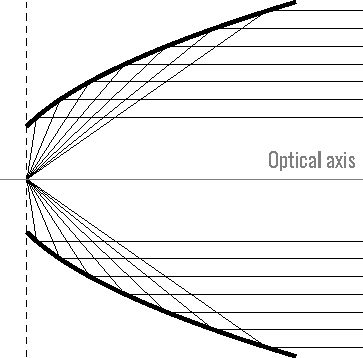
\includegraphics{figs/parabola_vsf.pdf}
    \caption{Typical VSF parabola, where the focal point is inside the
             mirror. The back of the parabola is cut up to the focal
             plane to remove to prevent light rays to reflect back
             into the laser chain.}
    \label{fig:vsf-v-hna.vsf}
  \end{subfigure}
  \caption[Illustrations of the typical HNA and VSF parabolas.]
          {Illustrations of typical HNA and VSF parabolas. For each
          parabola, the focal plane is indicated with a dashed line.
          The lines represent light rays that are specularly reflected
          by the surface. We can clearly see the one-point focus property
          of the parabolic mirror.}
  \label{fgi:vsf-v-hna}
\end{figure}

In this thesis, we implement solution (2) for most of our calculations, as
it is the one that entails less risk for the laser system. Depending on the focal
length, this can greatly reduce the proportion of the energy of the incident
beam that ends up in the focal spot, due to clipping. However, as we will
see, this configuration can be very advantageous in the observation of SF-QED
observables.

Before studying these observables, however, let's took a look at the behaviour
of the field as a function of $\alpha$.

\todo[inline]{Graph of ellipticity of electric intensity as a function of $\alpha$.}
\todo[inline]{Graph of waist size as a function of $\alpha$.}
\todo[inline]{Graph of max E and H intensity as a function of $\alpha$.}

  \begin{figure}
    \begin{subfigure}{0.47\textwidth}
      \centering
      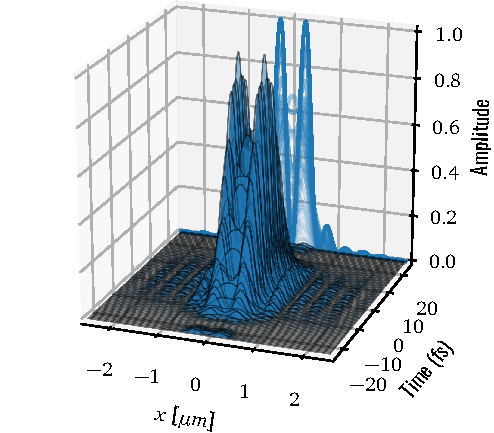
\includegraphics[width=\textwidth]{figs/ElectricIntensityTimeWaterfallf0.007.pdf}
      \caption{Electric intensity in the $x$ plane as a function of time for a parabola of $f=7\si{\milli\metre}$.}
      \label{fig:sc.electric_intensity_waterfall7}
    \end{subfigure}
    \hfill
    \begin{subfigure}{0.47\textwidth}
      \centering
      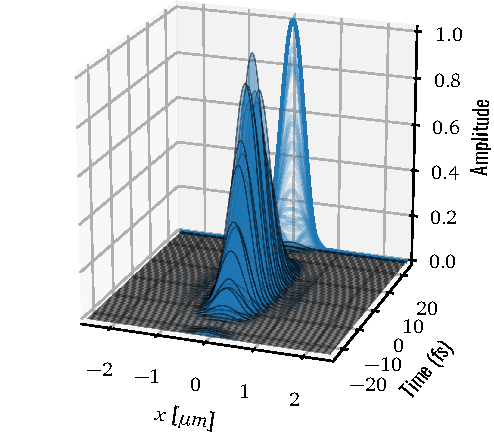
\includegraphics[width=\textwidth]{figs/ElectricIntensityTimeWaterfallf0.04375.pdf}
      \caption{Electric intensity in the $x$ plane as a function of time for a parabola of $f=43.75\si{\milli\metre}$.}
      \label{fig:sc.electric_intensity_waterfall43}
    \end{subfigure}
    \caption[Transverse cut of the electric intensity in the focal plane as a function of time, $x$ plane.]
            {Electric intensity in the $x$ plane as a function of time for different parabolas.
            Amplitude in arbitrary units. Each time slice is projected on the back of the figure.
            The line with the maximum intensity is opaque, and the opacity decreases as time
            goes away from zero, in both the positive and negative directions. Note that that at
            low values of $\alpha$, the longitudinal component $E_z$ dominates and the maximum
            of the intensity is found in lateral lobes and not at the focal point. At
            larger values of $\alpha$, the more typical Gaussian beam pattern is observed.}
    \label{fig:sc.electric_intensity_waterfall}
  \end{figure}

\todo[inline]{Analysis of analytical solutions in Appendix to interpret the tightly focused
fields.}


\todo[inline]{3D visualization of the tranverse part of the beam.}
\todo[inline]{3D visualization of the longitudinal components of the beam.}
\todo[inline]{Importance of the longitudinal component as a function of the focal length
                and its possible effects on SF-QED observables (FORESHADOWING).
                Interpretation of strong longitudinal components as presence
                of both forward and backwards propagating longitudinal vectors
                as focal length decreases.}
\todo[inline]{Confirm of infirm http://iopscience.iop.org/article/10.1088/2040-8986/aaadc8/meta.}

\subsection{Longitudinal Components}

\todo[inline]{Relative strength of the longitudinal component as a function of the
focal length.}

\subsection{Gouy Phase}

\todo[inline]{Gouy phase of tightly focused fields (deviation from Gaussian Gouy phase).}
\todo[inline]{Mention analytical solution for linear polarization.}
\todo[inline]{Computation of phase from 2D Fourier transforms.}

\subsection{Generation of Pseudo-Radial Beams with Mosaics}

\todo[inline]{Is this section worth it? Basically mention that since the
SC equations are linear, the articles on focused mosaics are still good.
Perhaps mention B-integral issues with thick broadband waveplates?
Find bandwidth at which the field is properly collimated? (This probably
can be done with the unfocused beams, so probably not interesting.)}


\section{Comparisons with Other Field Models}

As implied in the sections above, calculations using our Stratton-Chu implementation
can be quite long, in some cases taking up to five days! It is thus necessary
to make sure that the use of our formalism is indeed warranted. We will thus
compare the fields obtained with our method to other field models that appear in
the literature. We discuss both analytical solutions of Maxwell's equations
and the Richards-Wolf diffraction formalism.

For the sake of comparison, we will use a incident beam that has a Gaussian
spatial dependence, a super-Gaussian spectrum, and a parabola with a
numerical aperture of exactly 1. This produces a focused that is firmly
in the tight focusing regime, and allows for a comparison with a broad range
of field categories. See Table \ref{tab:comparison.parameters} for the exact
parameters.

\subsection{Analytical Field Models}

Another class of useful field models are vacuum solutions of the Maxwell equations.
In typical optical regimes, this is usually done via the paraxial approximation.
However, as we know, this approximation in invalid in the tight focusing regime.
It is possible, if more difficult, to write down solutions of Maxwell's equations
without this approximation. In this section, we will compare our StrattoCalculator
fields with those of the Salamin field model \cite{Salamin2015b}. This model purports to approximate
thtightly focused fields with only three free parameters: the central wavelength
of the radiation, its axial length, a parameter related to its temporal duration,
and the waist size.

The analytical expressions are relatively easy to numerically evaluate, although
there are two prominent issues. First, there doesn't seem to be a simple way
to evaluate the energy integral of these fields. Therefore, to fix the energy
content in this model, it is necessary to numerically integrate the field
over its whole spatial support with sufficient precision. In fact, for $w_0\ll L$,
fixing the energy content takes longer than subsequently evaluating the field.
Second, the expressions have singular behaviour around both $|\vb{r}|\sim0$ and $z=t$. Care must thus
be taken when evaluating the Salamin model in these regions.

Computing the fields in the focal plane, it is immediately apparent that this
model does not reproduce the high ellipticity that we observe in the fields
computed via the StrattoCalculator. Moreover, the relative strength of the
longitudinal components is much weaker than in the StrattoCalculator fields.
The origin of these discrepancies is quite simple: the analytical solution
cannot take into account the parabolic structure of the mirror. The phase
structures that the parabola imparts on the field has important consequences for
its focused properties.

Moreover, the Salamin model inherently cannot reproduce the fields produced
at $\alpha\ll1$. In this case, the parabolic shape is quite dramatic (in
more rigorous terms, it strongly diverges from a spherical mirror).
If we reduce the waist parameter, the longitudinal components become stronger,
but the primary field components never exhibit any ellipticity.

\subsection{The Richards-Wolf Formalism}

The Richards-Wolf formalism rests on two approximations. First, the focal point
is assumed far away from the reflecting surface, i.e. the far-field approximation
is used. The second one is less explicit and thus more difficult to trace:
it assumes that the light rays follow an energy conversation law.

In the focal region, the fields can be expressed as \cite{April2012}
  \begin{align}
    \vb{E}(r,\theta,z) &= \frac{1}{4\pi}\int_0^{2\pi}\int_0^{\alpha_\text{max}}
        \vb{E}_\text{sph}(\alpha,\beta)e^{-ikz\cos\alpha+ikr\sin\alpha\cos(\theta-\beta)}
        \sin\alpha d\alpha d\beta \\
    \vb{B}(r,\theta,z) &= \frac{1}{4\pi}\int_0^{2\pi}\int_0^{\alpha_\text{max}}
        \vb{B}_\text{sph}(\alpha,\beta)e^{-ikz\cos\alpha+ikr\sin\alpha\cos(\theta-\beta)}
        \sin\alpha d\alpha d\beta
  \end{align}
where
  \begin{align}
    \vb{E}_\text{sph} &= q(\alpha)\left[\vu{e}_\alpha\left(\vu{e}_\rho\cdot\vb{E}_\text{inc}\right)
                                       +\vu{e}_\beta\left(\vu{e}_\beta\cdot\vb{E}_\text{inc}\right)
                                       \right] \\
    \vb{H}_\text{sph} &= \left(\vu{e}_\alpha\times\vu{e}_\beta\right)\times\vb{E}_\text{sph}\nonumber\\
                      &= q(\alpha) \left[\vu{e}_\beta\left(\vu{e}_\rho\cdot\vb{E}_\text{inc}\right)
                                        -\vu{e}_\alpha\left(\vu{e}_\beta\cdot\vb{E}_\text{inc}\right)
                                        \right]
  \end{align}
where $\vu{e}_\alpha$ and $\vu{e}_\beta$ are the basis vectors of a spherical
coordinate system centered at the focal point.
We evaluate these from the parabola described above. We thus have
$\alpha_\text{max}=\pi/2$ and $q(\alpha)=\sec^2(\alpha/2)$.

We have implemented a simple C++ that evaluates these integrals for a single
frequency component of the electromagnetic field, but for arbitrary
apodization functions $q(\alpha)$ and arbitrary $\alpha$ limits.

We note that for the HNA.LIN.G.NA1 case, the Richards-Wolf formalism is virtually
indistinguishable from the Stratton-Chu results (Fig.\ref{fig:sc.sc-vs-rw-hna-lin-g-na1}).
We observe the same ellipticity on the primary components $E_x$ and $B_y$, and
similar magnitudes of the weaker transverse components and of the longitudinal
components. On that basis, we could tempted to conclude that both formalism yield
qualitatively the same results.

\begin{figure}
  \begin{subfigure}{\textwidth}
    \centering
    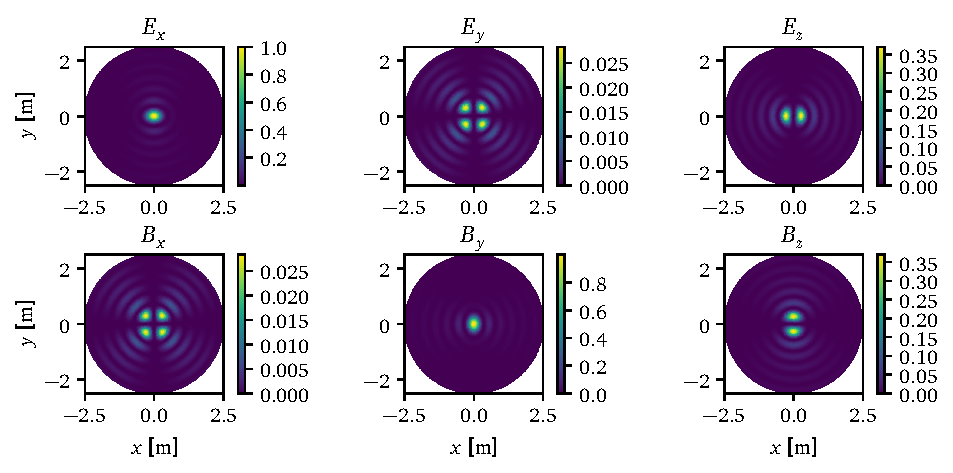
\includegraphics[width=\textwidth]{figs/RichardsWolf_fpNA1.pdf}
    \caption[Richards-Wolf field components for the HNA.LIN.G.NA1 case.]
            {Field components in the focal plane computed via the Richards-Wolf
            formalism for the parameters given in Table \ref{tab:comparison.parameters}}.
    \label{fig:sc.rw.hna-lin-g-na1}
  \end{subfigure}

  \begin{subfigure}{\textwidth}
    \centering
    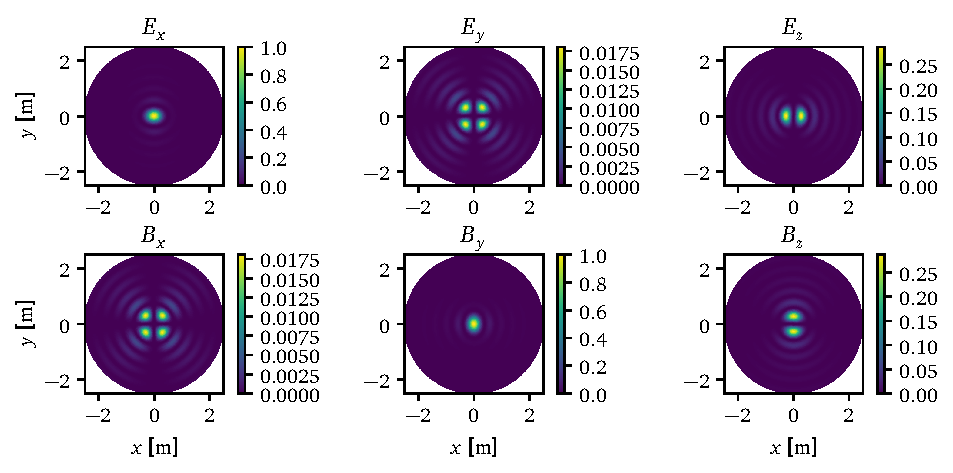
\includegraphics[width=\textwidth]{figs/StrattonChu_fpNA1.pdf}
    \caption[Stratton-Chu field components for the HNA.LIN.G.NA1 case.]
            {Field components in the focal plane computed via the Stratton-Chu
            formalism for the parameters given in Table \ref{tab:comparison.parameters}.}
   \label{fig:sc.sc.hna-lin-g-na1}
  \end{subfigure}

\caption[Richards-Wolf vs Stratton-Chu: fields in the focal plane, HNA.LIN.G.NA1.]
        {Comparison between the fields in the focal plane computed via
        the Richards-Wolf and the Stratton-Chu formalisms. Each plot represents
        the squared magnitude of a single Fourier component of the focused
        electromagnetic field.}
\label{fig:sc.sc-vs-rw-hna-lin-g-na1}
\end{figure}

However, when bringing the focal point inside the parabola, i.e. switching
to the VSF.LIN.G type, the two formalisms start to diverge (Fig.~\ref{fig:sc.sc-vs-rw-vsf-lin-g-f0.0875}).
The difference between the results of both formalisms increase with decreasing
focal length (Fig.~\ref{}). Insofar as we assume that the Stratton-Chu is the correct one,
an assumption that should be checked through experimentation, it seems that
the RW formalism underestimates the amount of energy that persists in the
focal spot, even at very small focal lengths.

\begin{figure}
  \begin{subfigure}{\textwidth}
    \centering
    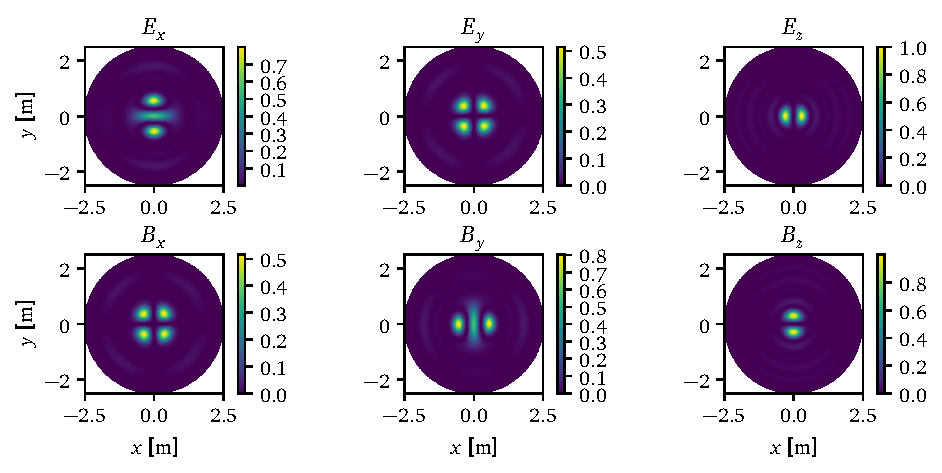
\includegraphics[width=\textwidth]{figs//RichardsWolf_fpVSF.pdf}
    \caption[Richards-Wolf field components for the VSF.LIN.G.f0.00875 case.]
            {Field components in the focal plane computed via the Richards-Wolf
            formalism for the parameters given in Table \ref{tab:comparison.parameters}}.
    \label{fig:sc.rw.vsf-lin-g-na1}
  \end{subfigure}

  \begin{subfigure}{\textwidth}
    \centering
    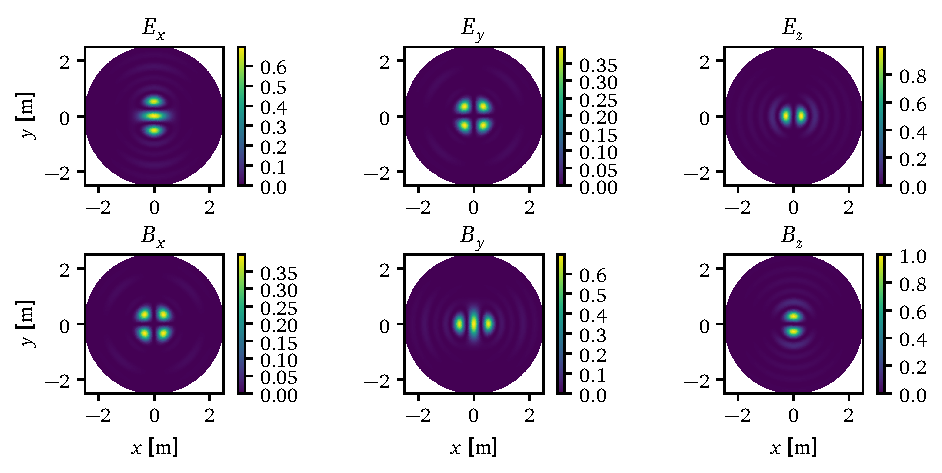
\includegraphics[width=\textwidth]{figs/StrattonChu_fpVSF.pdf}
    \caption[Stratton-Chu field components for the VSF.LIN.G.f0.00875 case.]
            {Field components in the focal plane computed via the Stratton-Chu
            formalism for the parameters given in Table \ref{tab:comparison.parameters}.}
   \label{fig:sc.sc.vsf-lin-g-f0.0875}
  \end{subfigure}

\caption[Richards-Wolf vs Stratton-Chu: fields in the focal plane, VSF.LIN.G.f0.00875.]
        {Comparison between the fields in the focal plane computed via
        the Richards-Wolf and the Stratton-Chu formalisms. Each plot represents
        the squared magnitude of a single Fourier component of the focused
        electromagnetic field.}
\label{fig:sc.sc-vs-rw-vsf-lin-g-f0.0875}
\end{figure}

\todo[inline]{Do we know of any reason for this? I would venture that
not taking into account the exact shape of the mirror would explain
this, as a spherical shape could maybe explain that effect.
(Check longitudinal fields https://en.wikipedia.org/wiki/Spherical\_aberration ).}

\todo[inline]{Statement of the RW formalism. Comment on derivation from RW to ST.}

\subsection{Numerical Verifications}

In this section, we study the convergence properties of our numerical implementation,
specifically in the evaluation of the integrals in Eq.~\eqref{eq:sc.stratton-chu-poa}.
We also verify that the reflected field have the same energy content as the incident
field, and that they obey Maxwell's equations.

These last two verifications are crucical in our case, as I am not aware of any
useful closed-form solutions of the Stratton-Chu equations that could be used
to compare to our numerically computed fields.

To study the convergence properties, we use our code to model the reflection
of a temporally short, radially polarized beam Gaussian beam with beam waist
$w_0$ and central wavelength $\lambda_c$. Its power spectrum is assumed to
have a super-Gaussian shape
  \begin{equation}
    \epsilon(\lambda) \propto \exp\left[-\left(\frac{\lambda-\lambda_c}{\Delta\lambda}\right)^{2n}\right].
  \end{equation}
The reflecting mirror is a paraboloid with focal length $f$ and aperture
radius $r_\text{max}$.
All the relevant parameters are shown in Table \ref{tab:comparison.parameters}.
\begin{table}
  \centering
  \begin{tabular*}{0.6\columnwidth}{@{\extracolsep{\fill} }lSc|lSc}
    \toprule
    \multicolumn{6}{c}{\textbf{Simulation Parameters}} \\
    \midrule
    \multicolumn{3}{c|}{Parabola}  & \multicolumn{3}{c}{Incident Beam}\\
    Param.           & {Value}     & Unit              & Param.          & {Value}     & Unit                 \\
    \midrule
    $r_\text{max}$   & 87.50       & \si{\milli\metre} & $w_0$           & 75          & \si{\mm}          \\
    $f$              & 43.75       & \si{\milli\metre} & $\lambda_c$     & 800         & \si{\nano\metre}     \\
                     &             &                   & $\Delta\lambda$ & 60          & \si{\nano\metre}     \\
                     &             &                   & $n$             & 4           &  --                  \\
                     &             &                   & $E_\text{tot}$  & 13.5        & \si{\joule}          \\
    \bottomrule
  \end{tabular*}
  \caption[Simulation parameters used in the convergence tests (radial polarization).]
          {Simulation parameters used in the convergence tests. The waist of the beam
          is chosen to minimize clipping, wherein the beam extends beyond the edge of the parabola,
          and the other parameters are typical of a broad spectrum, high-power laser.}
  \label{tab:comparison.parameters}
\end{table}

To gauge the convergence of our code, we compute the fields in the focal spot
for different mesh sizes on the paraboloid mirror. We use the finest mesh
as a reference and study the evolution of the relative difference between
the results as a function of the mesh size, i.e.
  \begin{equation}
    e_\text{rel}(N) = \frac{\max_{\vb{r}'}|F_{N_{r,\text{max}}}-F_{N}|}
                            {\max_{\vb{r}'}|F_{N_{r,\text{max}}}|}
  \end{equation}
where $\vb{F}_{N_r}$ is the electromagnetic field computed with $N_r$
radial discretization points. In cylindrical coordinates, unfortunately,
the cells are of nonuniform area across the mesh. We choose to use the average
area of the cells as a measure of mesh size, i.e.
  \begin{equation}
    \mean{A}_N = \frac{\Delta\theta(\Delta r)^2}{2}\sum_{n=0}^{N_r} (2n+1)
               = \frac{\Delta\theta(\Delta r)^2}{2}\frac{(N_r+1)^2}{N_r}
  \end{equation}

The computed electromagnetic fields via our implementation converge as
$(\text{average cell length})^4$, corresponding to the order of the
integration routine used in the test (Fig.~\ref{fig:sc.convergence-radial}).
The energy of the incident beam is also conserved by our code (Fig.~\ref{fig:sc.convergence-radial}d).

\begin{figure}
  \centering
  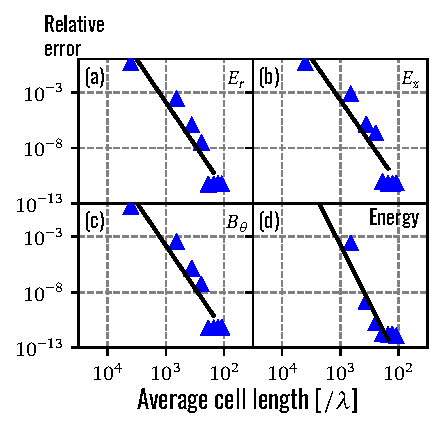
\includegraphics{figs/ConvergenceAll.pdf}
  \caption[Convergence pro
  perties of our Stratton-Chu implementation (radial polarization).]
  {Convergence properties of our Stratton-Chu implementation for a radially polarized
  incident beam. All components converge with $(\text{average cell length})^4$,
  i.e. with the order of the integration used in this test.}
  \label{fig:sc.convergence-radial}
\end{figure}

\todo[inline]{Verify that the numerically computed fields solve the Maxwell equations.}

\section{Partial Conclusion}

\todo[inline]{SC mostly used to model the fine details of tightly focused fields in an
experimental settings. Most easily used with fast SF-QED observable codes
in constract with PIC codes due to their high numerical cost.

Alternatives: propagation equations, transformation optics?}

\begin{comment}

IDEAS:
  \begin{itemize}
    \item Example of laser chain diagram with regime of validity of paraxial approximation.
    \item HNA parabolic mirror as counterexample in the laser chain, and danger of
            sending the laser back into itself through secondary reflections.
    \item Overlap of "focused" Gaussian beam with StrattoCalculator result.
    \item Overlap of other field models with StrattoCalculator.
  \end{itemize}

Skeleton:
  \begin{itemize}
      \item Short derivation of the Stratton-Chu equations, with emphasis on the physical optics approximation.
      \item Numerical implementation of the method
        \begin{itemize}
            \item Pros/cons vs more popular methods.
            \item Details of the field calculation (field models, normalization and whatnot).
            \item Details of the MPI implementation.
            \item Phase cancellation in the focal spot.
            \item Appendix: Numerical checks like convergence, solution of Maxwell's equations.
            \item Appendix: Far-field of the SC equations.
            \item Appendix: Analysis of the Gouy phase and its transverse momentum interpretation.
        \end{itemize}
      \item Comparison with Richards-Wolf:
        \begin{itemize}
            \item No ``real'' derivation from SC to RW without implicit approximations.
            \item Problem with phase cancellation?
            \item Differing results in similar conditions.
        \end{itemize}
      \item Analysis of the fields in the focal spot and comparison with
            existing analytical solutions (Salamin, e-dipoles).
      \item Opening to other methods that are less computationnaly intensive;
        \begin{itemize}
            \item Transformation optics;
            \item Propagation equations?
        \end{itemize}
  \end{itemize}

\end{comment}

\chapter{Application I: Four-Wave Mixing \textit{in vacuo} and Pair Production}
\label{chapter:fwm}

Application of tightly focused field model on observing SF-QED observables.
Can model realistic experimental configurations.

\todo[inline]{On the importance of modeling spatial inhomogeneities:
https://journals.aps.org/pra/abstract/10.1103/PhysRevA.97.022515}

Usual apparatus of SF-QED can be unwieldy to write down predictions in
complicated fields. Use of effective field theory to use ``first quantized''
theory that can easily accommodate complex fields. [Battesti, Dunne].

Most predictions rely on simple field models to be able to evaluate integrals [Karbstein].
Counterpoint, VEV theory by Karbstien that we should compare against.

% Skeleton:
% \begin{itemize}
%     \item Simple derivation of the EH Lagrangian.
%     \item How to extract FWM from EH: linearisation + integral solution (WaveMixer)
%     \item How to extract PP from EH: Adiabatic formula.
%     \item MASTER TABLE, or how different field models affect FWM.
%       \begin{itemize}
%         \item Introduction of the different field models.
%         \item Introduction of the transmission parabola.
%         \item Explain the behaviour of yield as a function of 2f/rmax with Lorentz invariants,
%               i.e. the optics of the experiment.
%       \end{itemize}
%     \item Pair production, w/ linear and radial beams.
%       \begin{itemize}
%           \item Show that both polarizations show the same behaviour as a function of f.
%           \item Visualize the 3D fields and explain optimum in terms of the optics (cancellation of the
%                 magnetic field in both cases).
%       \end{itemize}
% \end{itemize}

\section{Modelling Four-Wave Mixing in Strong, Classical Fields}

Short introduction of predictions of FWM by Euler, Kochel and Heiserberg.
Derivations of the effective field theory by Dunne. Corrections to Maxwell
equations. Limits of formalism and whatnot.

\todo[inline]{Unitarity of box diagram. https://arxiv.org/pdf/1805.00984.pdf}

\section{Four-Wave Mixing With Tightly Focused Fields}

Multiple experimental setups have been proposed in the FWM literature, with
the most common setup involving the collision of multiple beams at at angle.
In this thesis, we propose an alternative setup based on the tight focusing
a single laser pulse. This has the advantage of being simpler, and involving
less optical elements, and therefore of retaining the most energy in the
incident laser beam. However, it is much less flexible, as there are less
degrees of freedom in the control of the emission properties of the radiation
to be observed.

Our goal is to optimize the number of FWM photons that can readily be detected
in an all-optical experiment by tweaking the properties of the mirror and the
spectral and spatial properties of the single incident laser beam. The total
energy of the beam is fixed by the laser chain, although it is possible to change
the polarization and the wavefront of the beam, and, to some degree, its spatial
shape.

To this end, we will try to differentiate the total number of \textit{in vacuo}
FWM photons emitted and the observable number of photons. The exact definition
of observable will unfortunately depend on the experimental configuration
under study, but should provide an adequate measure of quality for our
purposes.

Four-wave mixing generates two types of frequencies. The dominant effect
is the broadening of the frequency spectrum of the incident beam, generated
by the first term of Eq.~\ref{}, and the second effect is third harmonic generation.
The latter has the advantage of being in a completely seperate bandwidth range
than the incident laser beam. However, there are numerous sources of noise in the
experiment that produce a similar third harmonic signal, such as four-wave mixing
on optical components (solids), imperfect vacuum that can lead to plasma formation,
and even simple Liénard-Wiechert emission (confirm in Chapter 3).

This chapter is structured as follows. We first compare the more typical
experimental setups available for single beam setups: the off-axis and
on-axis parabolic mirrors. \textbf{Summary of results.} We then explore
less typical parabolic mirrors, where the focal plane is inside the mirror
instead of outside. This configuration yields the most photons, but the
photons are harder to experimentally measure. This configuration has the
major problem that it creates backreflections that go directly back into the
laser chain, essentially destroying the laser chain. To avoid that, we remove
the part of the parabolic mirror that creates those reflections. This still
yields an optimal focal length, but even fewer photons. Finally, we explore
masking the incident field to create artifical shadows in the far-field where
FWM photons are emitted.

Description of the numerical algorithm to compute FWM.

\paragraph{Notation used in this chapter}

To simplify the presentation of the results, we will use abbreviations for
the different configurations we will explore. They are explained in
Table \ref{tab:fwm.setups-abbreviations}.

\begin{table}
  \begin{tabular}{cr}
    \toprule
    \multicolumn{2}{c}{\textbf{Geometry}} \\
    \midrule
    HNA & high numerical aperture parabola \\
    OFF & off-axis parabolic mirror \\
    VSF & transmission parabola, i.e. parabola with short focal length and cut at focal plane. \\
    \midrule
    \multicolumn{2}{c}{\textbf{Polarization}} \\
    \midrule
    LIN & linear polarization \\
    RAD & radial polarization \\
    MOS[N] & linearly polarized beam passed through a mosaic with N quadrants \\
    \midrule
    \multicolumn{2}{c}{\textbf{Field Shape}} \\
    \midrule
    G   & gaussian beam \\
    SG  & super-gaussian beam \\
  \bottomrule
  \end{tabular}
  \caption{Keys used throughout the chapter to denote the different parameters
           explored in the simulations.}
  \label{tab:fwm.setups-abbreviations}
\end{table}

\subsection{First Steps: On-Axis Parabola}

Most high-power lasers are set up with off-axis mirrors, as they are much
easier to align and cannot possibly reflect the laser beam back into the
chain. From a ray optics perspective, we expect the on-axis configurations
to reflect the beam back the same propagation axis regardless of focal length,
while the off-axis configurations to reflect at an angle that depends on the focal
length of the parabola and on the shift of the beam relative to the symmetry
axis of the full parabola.
The exact geometry of an off-axis parabolic mirror used in this thesis
is shown in Fig.~\ref{fig:fwm.geometry-of-off-axis-setup}.

\begin{figure}
  \centering
  \begin{subfigure}[t]{0.49\textwidth}
    \centering
    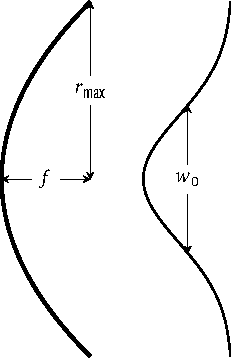
\includegraphics{figs/onaxis-parabola.pdf}
    \caption{On-axis configuration.}
    \label{fig:fwm.on-axis-geometry}
  \end{subfigure}
  \hfill
  \begin{subfigure}[t]{0.49\textwidth}
    \centering
    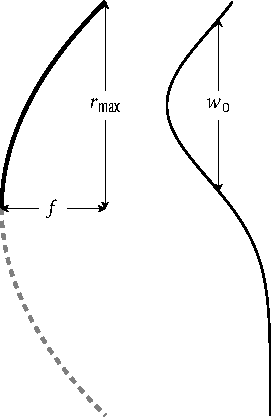
\includegraphics{figs/offaxis-parabola.pdf}
    \caption{Off-axis configuration.}
    \label{fig:fwm.off-axis-geometry}
  \end{subfigure}
  \caption[Schematic representation of the on- and off-axis configurations.]
          {Schematic representations of the \textbf{(a)} on-axis and \textbf{(b)}
          off-axis configurations. In the on-axis configuration, the incident field is aligned with
          the geometric center of the parabola, i.e. the maximum of the field coincides with
          the symmetry axis of the parabola. In the off-axis case, only a portion of a typically
          larger parabola is used, and the incident beam is aligned with the center of the partial
          parabola.}
  \label{fig:fwm.geometry-of-off-axis-setup}
\end{figure}

However, even at their tighter focus, they yield less photons than their on-axis
counterparts (Table \ref{tab:fwm.hna-lin-g}). The lack of symmetry of the setup
is manifest in the angular spectrum angular radiation (Fig.~\ref{fig:fwm.hna-vs-off}).
This could be advantageous however, as most of the emission is in the sidelobes around
the peak of the reflected laser beam.

\begin{figure}
  \centering
  \begin{subfigure}{0.49\textwidth}
    \centering
    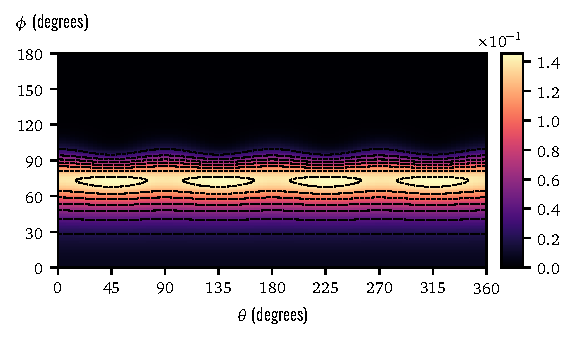
\includegraphics[width=\textwidth]{figs/fwm_hna1_angspec_f_cont.pdf}
    \caption{Photon angular spectrum in the HNA.LIN.G with $\alpha=1$.}
    \label{fig:fwm.hna-lin-g-1.0}
  \end{subfigure}
  \hfill
  \begin{subfigure}{0.49  \textwidth}
    \centering
    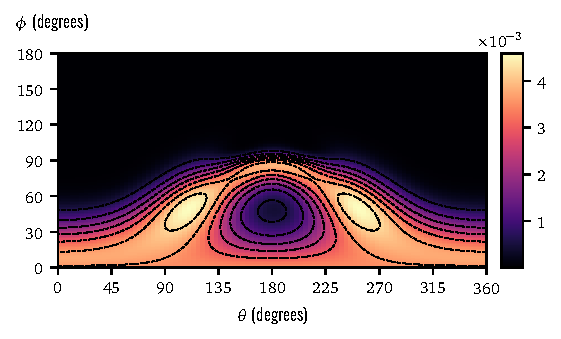
\includegraphics[width=\textwidth]{figs/fwm_off1_angspec_f_cont.pdf}
    \caption{Photon angular spectrum in the OFF.LIN.G with $\alpha\sim0.96$.}
    \label{fig:fwm.off-lin-g-0.96}
  \end{subfigure}
  \caption[Angular spectra of the first harmonic photons generated by \textit{in vacuo} FWM.]
          {Photon angular spectra of the first harmonic generated by
          \textit{in vacuo} four-wave mixing. Note the higher divergence
          and degree of symmetry in \textbf{(a)} compared to \textbf{(b)}.
          The off-axis parabola produces asymmetrical Lorentz invariants and,
          in turn, a highly inhomogeneous angular spectrum.}
  \label{fig:fwm.hna-vs-off}
\end{figure}

On-axis configurations, for their part, deliver a highly symmetric emission
spectrum, but that co-propagates with the incident laser beam, complicating
detection. \todo{Would it be feasible to have the far-field of the linearly
polarized beam easily?}

In this case, it is hard to make a distinction between the total number of photons
and the number of observable photons, as we do not readily have access to the
far-field emission patterns of the reflected beam in the OFF.LIN.G case.
\todo{Can we even have access to the HNA.LIN.G one?}


\subsection{Varying the Focal Length}

Varying the focal length of on-axis parabolic mirrors, allowing the focal
spot to be inside of the mirror geometry itself ($\alpha\leq1$) reveals that
there exists an optimum focal length value. Its exact value, of course, depends
on the parameters of the simulation. However, it seems to robustly lie in the
range $\alpha\sim0.3--0.5$ for linearly or radially polarized beam, with Gaussian
or super-Gaussian spatial shape and for HNA and VSF parabolas.

The root cause of this optimum is the interplay between the effective volume
of photon creation and the maximum values of the polarization and magnetization.
Indeed, all the relevant quantities that describe vacuum FWM, i.e. the Lorentz
invariants $\mathcal{F}$ and $\mathcal{G}$, the reduced invariants $\mathcal{E}$
and $\mathcal{H}$, are all maximum at $\alpha=1$ while the actual number of
photons increases up to $\alpha\sim0.38$ (in the HNA.LIN.G case).

This increase in the volume of photon creation also causes a broadening of
the angular spectrum in the $\phi$ direction. We surmise that this is due
to the higher spread of electromagnetic field $\vb{k}$ vectors that contribute
to photon creation.\todo{It is possible to show that by Fourier transforming
the fields or something?}

Another consequence of shortening the focal length is to increase the angle
at which the photons are emitted (Fig.~\ref{}). For $\alpha\geq1$, this can simply
be explained by the fact that as the focal length decreases, the field becomes
more tightly focused and hence more divergent. Following the divergence of the
incident beam, the FWM photons are emitted at a sharper angle. For $\alpha\leq1$,

Unfortunately, such a geometry is difficult to implement in practice. The portion
of the parabola that is behind the focal plane reflects the laser beam back
into the laser chain and risks damaging it. A simple solution to this conundrum
is to simply remove, i.e. cut away, this portion of the parabola. The immediate
problem that we face is that, barring any modification of the incident beam,
clips away the central portion of the incident beam.

Nevertheless, this geometry proves to be a promising one, generating almost
the same total number of photons as the HNA.LIN.G($\alpha=1$) configuration.
To assess its relative worth, we define an observable number of photons
for each of these geometries.

The VSF configuration type defines a natural ``shadow'' in the far-field
pattern, as can be seen from simple ray optics (Fig.~{}). Experimentally, it is
possible to place a detector in this shadow to facilitate the detection of FWM
photons. The observable number of photons, then, is simply the integral of the
angular spectrum in this shadow.

To compare the VSF and HNA configurations, we induce an artificial shadow in
the HNA parabola by masking the center of the beam with a circular absorber
of a given size. The larger the mask, the larger the shadow. The interplay
between the energy absorbed by the mask and the size of the shadow creates
an optimal value for the mask size. We compare the natural shadow of the VSF
with the optimal shadow of the HNA.

\todo[inline]{Charts with number of photons for each.}

\definecolor{phd_orange}{HTML}{FFB14E}
\renewcommand{\chart}[1]{
  \ChartBox{#1}{0.22\textwidth/6.09*#1}{phd_orange}}

\todo[inline]{Fix the colours of the chart. Fix the large negative sign.}

\begin{table}
  \centering
  \begin{tabularx}{0.66\textwidth}{@{\extracolsep{\fill}}S[table-format=1.5E+2,output-exponent-marker=\text{E},mode=text]%
                                   @{\extracolsep{\fill}}S[table-format=1.2,mode=text]%
                                   p{0.22\textwidth}}
  \toprule
  \multicolumn{3}{c}{HNA.LIN.G}\\
  \midrule
  \multicolumn{1}{c}{$2f/r_\text{max}$} & \multicolumn{1}{l}{$f\;[\si{\mm}]$} & Number of photons (1st) \\
  \midrule
  2.28571E-02       & 1                 & \chart{1.15321E-04}  \\
  1.14286E-01       & 5                 & \chart{2.07763E-01}  \\
  2.05714E-01       & 9                 & \chart{1.70786E+00}  \\
  2.74286E-01       & 12                & \chart{3.64066E+00}  \\
  3.88571E-01       & 17                & \chart{6.09274E+00}  \\
  5.02857E-01       & 22                & \chart{5.90221E+00}  \\
  6.17143E-01       & 27                & \chart{4.11350E+00}  \\
  7.31429E-01       & 32                & \chart{2.38156E+00}  \\
  8.45714E-01       & 37                & \chart{1.28552E+00}  \\
  1.00000E+00       & 43.75             & \chart{5.65765E-01}  \\
  1.59634E+00       & 69.84             & \chart{3.77655E-02}  \\
  2.00137E+00       & 84.56             & \chart{8.42140E-03}  \\
  2.45714E+00       & 107.5             & \chart{1.98551E-03}  \\
  \midrule
  \multicolumn{3}{c}{OFF.LIN.G}                                \\
  \midrule
  9.56363E-01       & 78.9             & \chart{1.22234E-02} \\
  \bottomrule
  \end{tabularx}
  \caption{Number of photons as a function of the focal length $f$
           of a parabolic mirror. The incident field has a Gaussian
           spatial shape. The aperture size is fixed at $
           r_\text{max}=87.50\,\si{\mm}$ for the HNA.LIN.G configurations
           and $r_\text{max}=165\,\si{\mm}$ for the OFF.LIN.G configuration.}
  \label{tab:fwm.hna-lin-g}
\end{table}

\subsection{Maximing the Observable Number of Photons}

To optimize the probability of detecting four-wave mixing in vacuum, it is
necessary to increase the relatively low number of detectable photons. Up to
this point, we have changed the geometry of the reflecting surface and the polarization
properties of the beam to increase the total number of photons generated.
In this section, we will instead try to increase the number of observable photons
in each configuration.

In the previous section, we saw that the natural shadow of the VSF and the
artificial shadow of the HNA unfortunately do not intersect with the bulk
of the photon density. Instead of using a simple centered circular mask,
it is possible to mask another portion of the beam to create a shadow exactly
where the photon density is high (see Fig.~\ref{fig:fwm.vsf-v-hna} for a sketch).
For a maximal number of photons, an annular mask would be preferred. However,
it is harder to get annular detectors to actually recover all that information.
We will hence try circular or elliptical masks.

\begin{figure}
  \begin{subfigure}[t]{0.47\textwidth}
    \centering
    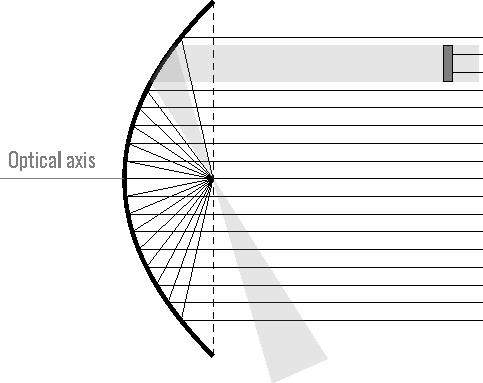
\includegraphics{figs/masked_parabola_hna.pdf}
    \caption{Masked HNA parabola.}
    \label{fig:vsf-v-hna.hna}
  \end{subfigure}
  \hfill
  \begin{subfigure}[t]{0.47\textwidth}
    \centering
    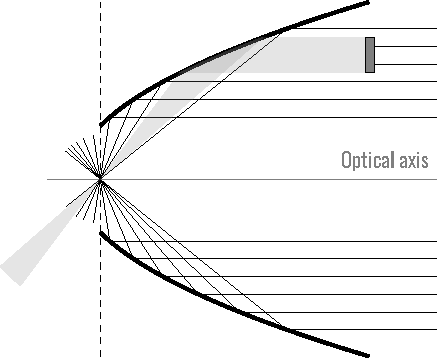
\includegraphics{figs/masked_parabola_vsf.pdf}
    \caption{Masked VSF parabola.}
    \label{fig:vsf-v-hna.vsf}
  \end{subfigure}
  \caption[Illustrations of the masked HNA and VSF parabolas.]
          {Illustrations of masked HNA and VSF parabolas.}
  \label{fig:fwm.vsf-v-hna}
\end{figure}

\todo[inline]{Compare results and presentation with
https://journals.aps.org/prd/abstract/10.1103/PhysRevD.97.036022.}

\todo[inline]{Compare results and presentation with
https://journals.aps.org/prd/pdf/10.1103/PhysRevD.97.036026.}

\todo[inline]{Comparison with dynamical assistance. https://journals.aps.org/prd/pdf/10.1103/PhysRevD.97.096004}

\chapter{Application II: Radiation of Charged Particles in Tightly Focused Fields}
\label{chapter:electron_trajectories}

Skeleton (still a rough idea):
  \begin{itemize}
    \item Quantify RR in different field configurations, checking whether there
          is an advantage to using a transmission parabola in this case.
    \item Study the effects of different field models on the detectability of
          RR effects.
    \item Mention intensity measurement stuff? I've worked a little on this\ldots
  \end{itemize}

\todo[inline]{See https://journals-aps-org.acces.bibl.ulaval.ca/prd/pdf/10.1103/PhysRevD.97.105001
for important parameters.}

\todo[inline]{Perspectives: QED transition amplitudes in plasmas.
https://arxiv.org/abs/1805.01762}

\chapter{Conclusion}

\section{Summary of contributions}

\section{Further optimization of beam profiles}

\section{Better modeling of noise through plasma simulations}

\appendix
\addtocontents{toc}{\protect\setcounter{tocdepth}{0}}
%\addtocontents{toc}{\addtolength\cftchapternumwidth{\widthof{Appendix\;}}}
\renewcommand{\thechapter}{\Alph{chapter}}
\renewcommand{\thesection}{\Alph{chapter}.\arabic{section}}
\chapter{Evaluation of the Singular Surface Integrals in the Stratton-Chu Diffraction Integrals}
\label{app.limits}


Here, we evaluate the singular part of the integrals of the Stratton-Chu equations,
Eqs.~\eqref{eq:sc.singularLimits}.
The integration is done over a hemispherical surface of radius $R$ centered at
$\vb{r}=\vb{r}'$. We use spherical coordinates $(R,\phi,\theta)$. Note that
$\vb{R}=\vb{r}-\vb{r}'$ in these coordinates.
We then take the limit as $R\rightarrow0$. Since the surface
is small, we suppose that the field does not change on the surface and assume
it takes its value at $\vb{r}=\vb{r}'$ over the whole surface. We can then move it
outside the integral sign. We also ignore the phase of the Green's function, as
it is constant over the hemisphere and goes to 0 after the limit.
The integral over the hemisphere in Eq.~\eqref{eq:sc.regularLimit} becomes
  \begin{align}
    \lim_{R\rightarrow0}\iint_{S_\epsilon}\vb{A}gdS
      &= \lim_{R\rightarrow0}\vb{A}\int_0^{\frac{\pi}{2}}\int_0^{2\pi}\frac{1}{4\pi R} R^2 \sin\theta d\phi d\theta,\nonumber\\
      &= 0.
  \end{align}
The integral is in fact regular at $\vb{r}=\vb{r}'$ because the integration measure
cancels the pole of the Green's function.

In Eq.~\eqref{eq:sc.singularLimit}, the gradient of the Green's function
generates a $R^{-1}$ term and a $R^{-2}$ term. The former does not contribute to the integral
because of the integration measure, while the latter reads
  \begin{align}
    \lim_{R\rightarrow0}\iint_{S_\epsilon}\vb{A}\times\nabla gdS
      &= \lim_{R\rightarrow0}\vb{A}\times
      \int_0^{\frac{\pi}{2}}\int_0^{2\pi}\frac{R^2\vu{n}}{4\pi R^2}\sin\theta d\phi d\theta, \nonumber\\
      &= \frac{1}{2}\vb{A}\times\vb{n},
  \end{align}
where $\vb{n}$ comes from the fact that the gradient of the Green's function is
normal to the hemispherical surface.

The integral in Eq.~\eqref{eq:sc.hypersingularLimit} diverges due to the presence
of the double gradient of $g$. However, it is still possible to assign it a finite
value.
To do so, we use the explicit
expression of the double gradient of the Green's function \cite[Eq. (2.61)]{Volakis2012}:
  \begin{align}
    \label{eq:singularInt.doubleGradientExp}
    \nabla\nabla g(\vb{r},\vb{r}')  &= -\dyad{I}\left[-\frac{ik}{R}+\frac{1}{R^2}\right]g
                    +\left(\vu{R}\otimes\vu{R}\right)\left[\frac{3}{R^2}-\frac{3ik}{R}-k^2\right]g
  \end{align}
where $\dyad{I}$ is the unit dyad, $R=|\vb{r}-\vb{r}'|$, $\vu{R}=(\vu{r}-\vu{r}')/R$
and $\otimes$ is the Kronecker outer product. The contribution of the second line
of Eq.~\eqref{eq:singularInt.doubleGradientExp} to the surface integral
vanishes due to the tensor structure, i.e.
  \begin{align}
    \label{eq:singularInt.dyadVectorProd}
    \vu{R}\otimes\vu{R}\cdot\left(\vu{n}\times\vb{F}\right)&\xrightarrow{r\in S_\epsilon}
      \vu{R}\otimes\vu{R}\cdot\left(\vu{R}\times\vb{F}\right).
  \end{align}
On the hemispherical surface, the dyad $\vu{R}\otimes\vu{R}$ has a single
non-vanishing component in, obviously, the $\vu{R}\otimes\vu{R}$ direction, while the vector
it multiplies, $\vu{R}\times\vb{F}$ only has angular ($\vu{\phi}$ and $\vu{\theta}$)
components. The dyad-vector product
of Eq.~\eqref{eq:singularInt.dyadVectorProd} thus
vanishes. The contribution of the first line of Eq.~\eqref{eq:singularInt.doubleGradientExp}, however,
does not vanish. We expand it in a Laurent-type series and obtain
  \begin{align*}
    \left(-\frac{ik}{R}+\frac{1}{R^2}\right)g
      &\simeq \left(-\frac{ik}{R^2}+\frac{1}{R^3}\right)\left(1+ikR\right) \\
      &= -\frac{ik}{R^2}+\frac{1}{R^3}+\frac{k^2}{R}+\frac{ik}{R^2} \\
      &= \frac{1}{R^3}+\frac{k^2}{R}.
  \end{align*}
Substituting this last expression in the l.h.s of Eq.~\eqref{eq:sc.hypersingularLimit},
we see that the second term vanishes due to the $R^2$ measure and that the
first term formally diverges. To ascribe a finite value to this integral,
we make use of the Hadamard finite part, which essentially drops the diverging term
in a mathematically consistent way \cite{Blanchet2000}.
Equation (\ref{eq:sc.hypersingularLimit}) thus reads
  \begin{equation}
    \lim_{\vb{r}'\in S} \iint_S \nabla\nabla g \cdot\left(\vu{n}\times\vb{F}\right)dS
     = \HadamardSurf_S \nabla\nabla g\cdot\left(\vu{n}\times\vb{F}\right)dS.
  \end{equation}

\chapter{Explicit expressions of the Stratton-Chu equations}
\label{app.explicit-sc}

In chapter \ref{chapter:stratton-chu}, we discussed the numerical evaluation
of the Stratton-Chu equations as a way to model electromagnetic fields in the
tightly focused regime. Specifically, we implemented a program that evaluates
\eqref{eq:sc.stratton-chu-poa-og} for arbitrary mirror geometries, arbitrary incident fields and capable
of modeling broadband pulses. In this appendix, we provide explicit expressions
of the Stratton-Chu equations in cylindrical coordinates and write down a far-field
approximation of those equations.

\section{Explicit expression in cylindrical coordinates}

Our starting point is \eqref{eq:sc.stratton-chu-poa-og}, which we print here for convenience
  \begin{subequations}
  \label{eq:app.sc-explicit.poa-og}
  \begin{align}
    \label{eq:app.sc-explicit.poa-og.efield}
    \vb{E}'_\text{ref}(\vb{r}',k)  &= 2\iint_S
      \left\{
        ik(\vu{n}\times\vb{B}_\text{inc})g
        +\left(\vu{n}\cdot\vb{E}_\text{inc}\right)\nabla g\right\}dS
            + \frac{2}{ik}\oint_{\partial S}\nabla g
                    \vb{B}\cdot d\vb{\ell},\\
                    %\left[\vu{n}\times(\vu{n}\times\vb{B}_\text{inc})\right]\cdot d\vb{\ell},\\
    \label{eq:app.sc-explicit.poa-og.bfield}
    \vb{B}'_\text{ref}(\vb{r}',k)  &= 2\iint_S (\vu{n}\times\vb{B}_\text{inc})\times\nabla g dS.
  \end{align}
  \end{subequations}
where recall that
  \begin{align}
    g(\vb{r},\vb{r}') &= \frac{e^{ik\left|\vb{r}-\vb{r}'\right|}}{\left|\vb{r}-\vb{r}'\right|}, \\
    \left|\vb{r}-\vb{r}'\right| &= \sqrt{r^2+r'^2-2rr'\cos(\theta-\theta')-(z-z')^2}.
  \end{align}

Before we proceed, we'll show some useful intermediate results that will ease the parsing
of this expression. First, note that we compute the gradient of the Green's
function w.r.t. to the unprimed coordinates such that
  \begin{equation}
    \nabla g = \left(\frac{ik}{u}-\frac{1}{u^2}\right)\left[\left(r-r'\cos(\theta-\theta')\right)\vu{r}+r'\sin(\theta-\theta')\vu{\theta}+(z-z')\vu{z}\right]g = \left(\frac{ik}{u}-\frac{1}{u^2}\right)g\vb{G}
  \end{equation}
Also note that to extract the cylindrical components of the electromagnetic
field vectors, it will be necessary to evaluate the dot product of
\eqref{eq:app.sc-explicit.poa-og} with cylindrical basis vectors evaluated
at $\vb{r}'$ with cylindrical basis vectors evaluated at $\vb{r}$.
Because the cylindrical basis vectors form a non-coordinate basis, these
dot products do not vanish. In fact, we have
  \begin{subequations}
  \begin{align}
    \vu{r}'\cdot\vu{r}            &= (\cos\theta'\vu{x}+\sin\theta'\vu{y})\cdot(\cos\theta\vu{x}+\sin\theta\vu{y})
                                   = \cos\theta'\cos\theta+\sin\theta'\sin\theta
                                   = \cos(\theta-\theta') \\
    \vu{r}'\cdot\vu{\theta}       &= (\cos\theta'\vu{x}+\sin\theta'\vu{y})\cdot(-\sin\theta\vu{x}+\cos\theta\vu{y})
                                   = -\cos\theta'\sin\theta+\sin\theta'\cos\theta
                                   = -\sin(\theta-\theta')\\
    \vu{\theta'}\cdot\vu{r}       &= (-\sin\theta'\vu{x}+\cos\theta'\vu{y})\cdot(\cos\theta\vu{x}+\sin\theta\vu{y})
                                   = -\sin\theta'\cos\theta+\cos\theta'\sin\theta
                                   = \sin(\theta-\theta') \\
    \vu{\theta}'\cdot\vu{\theta}  &= (-\sin\theta'\vu{x}+\cos\theta'\vu{y})\cdot(-\sin\theta\vu{x}+\cos\theta\vu{y})
                                   = \sin\theta'\sin\theta+\cos\theta'\cos\theta
                                   = \cos(\theta-\theta')
  \end{align}
  \end{subequations}

To streamline the computation, we first compute the vector products contained
in each term of the integrands individually. This yields
  \begin{align}
    \vb{N}\times\vb{B}_\text{inc}
                &= \left[
                \left(n_\theta B_z-n_z B_\theta\right) \vu{r}
                    +\left(n_z B_r-n_r B_z\right)      \vu{\theta}
                    +\left(n_r B_\theta- n_\theta B_r\right)  \vu{z}
                  \right] \\
    \vb{N}\cdot\vb{E}_\text{inc}
                &= n_r E_r + n_\theta E_\theta + n_z E_z \\
    (\vb{N}\times\vb{B}_\text{inc})\times\vb{G}
                &= \left\{
                      \left[
                        \left( n_z B_r - n_r B_z \right) G_z
                        -\left( n_r B_\theta - n_\theta B_r \right) G_\theta
                      \right] \vu{r} \right. \nonumber\\
                &\quad+\left[
                        \left( n_r B_\theta - n_\theta B_r \right) G_r
                       -\left( n_\theta B_z - n_z B_\theta\right) G_z
                      \right]  \vu{\theta} \nonumber\\
                &\quad+\left.\left[
                    \left( n_\theta B_z-n_z B_\theta \right) G_\theta
                    -\left( n_z B_r - n_r B_z \right) G_r
                      \right]\vu{z}\right\}
  \end{align}
We can now extract the explicit expressions for the components of the reflected
electromagnetic fields, paying attention to the products of primed and unprimed
basis vectors:
%\todo[inline]{Check for multiline automatic sizing for \verb|\left| and \verb|\right|.}
  \begin{subequations}
  \begin{align}
    E_r'(\vb{r}', k)
          &= \vu{r}'\cdot\vb{E}'(\vb{r}',k) \nonumber\\
          &= 2\iint_S\left\{ikg \left[
              \left( n_\theta B_z -n_z B_\theta \right)\cos(\theta-\theta')
              +\left(n_r B_z -n_zB_r \right)         \sin(\theta-\theta')\right]\right.\nonumber\\
            &\quad \left.+\left(\frac{ik}{u}-\frac{1}{u^2}\right)g
                   \left(n_r E_r + n_\theta E_\theta + n_z E_z\right)\left(r\cos(\theta-\theta')-r'\right)\right\}dS \nonumber\\
            &\quad + \frac{2}{ik}\oint_{\partial S} \left(\frac{ik}{u}-\frac{1}{u^2}\right) g
                    \left(B_r l_r + B_\theta l_\theta + B_z l_z\right)\left(r\cos(\theta-\theta')-r'\right)dl,\\
   E_\theta'(\vb{r}',k)
          &=\vu{\theta}'\cdot\vb{E}'(\vb{r}',k) \nonumber\\
          &= 2\iint_S\left\{ikg \left[
              \left(n_\theta B_z - n_z B_\theta\right)\sin(\theta-\theta')
              +\left(n_z B_r  - n_r B_z\right)        \cos(\theta-\theta')\right]\right.\nonumber\\
            &\quad+\left(\frac{ik}{u}-\frac{1}{u^2}\right)g\left.\left(n_r E_r + n_\theta E_\theta + n_z E_z\right)
             r\sin(\theta-\theta')g\right\}dS \nonumber\\
            &\quad +\frac{2}{ik}\oint_{\partial S} \left(\frac{ik}{u}-\frac{1}{u^2}\right)g
                    \left(B_r l_r + B_\theta l_\theta + B_z l_z\right)r\sin(\theta-\theta')dl \\
  E_z'(\vb{r}',k)
          &= \vu{z}'\cdot\vb{E}'(\vb{r}',k) \nonumber\\
          &= 2\iint_S\left\{ikg \left(n_r B_\theta - n_\theta B_r\right)+\left(\frac{ik}{u}-\frac{1}{u^2}\right)\left( n_r E_r + n_\theta E_\theta + n_z E_z\right)(z-z')g\right\} dS\nonumber\\
            &\quad +\frac{2}{ik}\oint_{\partial S} \left(\frac{ik}{u}-\frac{1}{u^2}\right)g
              \left(B_r l_r + B_\theta l_\theta + B_z l_z\right)(z-z')dl
  \end{align}
The magnetic field gives
  \begin{align}
    B_r'(\vb{r}', k)
          &= \vu{r}'\cdot\vb{B}'(\vb{r}',k) \nonumber\\
          &= 2\iint_S \left(\frac{ik}{u}-\frac{1}{u^2}\right)g \left[
                \left(n_z B_r - n_r B_z \right) (z-z')\cos(\theta-\theta')\right.\nonumber\\
          &\quad\left.\left(
               +r\left(n_\theta B_r - n_r B_\theta\right)
               +\left(n_\theta B_z - n_z B_\theta\right)(z-z')\right)\sin(\theta-\theta')
               \right] \\
    B_\theta'(\vb{r}',k)
          &=\vu{\theta}'\cdot\vb{B}'(\vb{r}',k) \nonumber\\
          &= 2\iint_S \left(\frac{ik}{u}-\frac{1}{u^2}\right)g \left[
              \left(n_z B_r-n_r B_z\right)(z-z')\sin(\theta-\theta')\right. \nonumber\\
          &\quad +\left(n_z B_\theta - n_\theta B_z\right)(z-z')\cos(\theta-\theta') \nonumber\\
          &\quad\left.+\left(n_\theta B_r- n_r B_\theta\right)\left(r'-r\cos(\theta-\theta')\right)\right] dA \\
    B_z'(\vb{r}',k)
          &= \vu{z}'\cdot\vb{B}'(\vb{r}',k) \nonumber\\
          &= 2\iint_S \left(\frac{ik}{u}-\frac{1}{u^2}\right)g\left[
            \left(n_\theta B_z- n_z B_\theta\right)r'\sin(\theta-\theta') \right.\nonumber\\
          &\quad\left.+\left(n_r B_z - n_z B_r\right)\left(r-r'\cos(\theta-\theta')\right)\right] dA
  \end{align}
  \end{subequations}

For the given parametrization, the normal is given
  \begin{subequations}
  \begin{align}
    \vu{n} &= \frac{\nabla(z-F(r,\theta))}{\left|\nabla(z-F(r,\theta))\right|} \\
           &= \frac{\left[-\partial_r F(r,\theta)\vu{r}-\frac{1}{r}\partial_\theta F(r,\theta)\vu{\theta}+\vu{z}\right]}
                    {\sqrt{1+\left(\partial_r F(r,\theta\right)^2+\left(\frac{1}{r}\partial_\theta F(r,\theta)\right)^2}}
  \end{align}
while the surface element is given by
  \begin{equation}
    dS = dA\sqrt{1+\left(\partial_r F(r,\theta)\right)^2+\left(\frac{1}{r}\partial_\theta F(r,\theta)\right)^2}.
  \end{equation}
  \end{subequations}
Given that the normal vector is present only once in most of terms of the integrals,
the Jacobian due to the surface will conveniently cancel.

\section{Far-Field Expressions}

When using the Stratton-Chu equations, our interest lies in computing fields
in the tight focusing regime. As such, we will generally compute the fields
in a small region around the focal spot. In practice, this means that the mirror
is far away from the region over which we compute the field­. The approximation
that $|\vb{r}|\gg|\vb{r}'|$ can thus be used to simplify the expressions.
This is akin to a far-field approximation, except that the observation point is
close to the origin instead of far from it: it is instead the source point that
is far away.

To simplify the procedure, notice that $\nabla g = -\nabla' g$, such that we
start from
  \begin{subequations}
  \begin{align}
    \vb{E}'_\text{ref}(\vb{r}',k)  &= 2\iint_S
      \left\{
        ik(\vu{n}\times\vb{B}_\text{inc})g
        -\left(\vu{n}\cdot\vb{E}_\text{inc}\right)\nabla' g\right\}dS
        -\frac{2}{ik}\oint_{\partial S}\nabla' g
                    \vb{B}\cdot d\vb{\ell},\\
                    %\left[\vu{n}\times(\vu{n}\times\vb{B}_\text{inc})\right]\cdot d\vb{\ell},\\
    \vb{B}'_\text{ref}(\vb{r}',k)  &= -2\iint_S (\vu{n}\times\vb{B}_\text{inc})\times\nabla' g dS.
  \end{align}
  \end{subequations}
Given our approximation, we can write
  \begin{equation}
    |\vb{r}-\vb{r}'| = R-\frac{1}{R}\vb{r}\cdot\vb{r}'
  \end{equation}
and
  \begin{equation}
    g(\vb{r},\vb{r}') = \frac{e^{ikR}}{R}e^{-\frac{ik}{R}\vb{r}\cdot\vb{r}'}
  \end{equation}
where $R=|\vb{r}|$. The gradient thus yield the simple expression
  \begin{equation}
    \nabla'g = -\frac{ikg}{R}\vb{r}
  \end{equation}
\todo[inline]{Fix the notation for $|\vb{r}|/R$. Right now it's confusing as all hell.}
Substituting yields
  \begin{subequations}
  \begin{align}
    E_r'(\vb{r}', k)
          &= 2ik\iint_S\left\{ \left[
              \left( n_\theta B_z -n_z B_\theta \right)\cos(\theta-\theta')
              +\left(n_r B_z -n_zB_r \right)         \sin(\theta-\theta')\right]\right.\nonumber\\
            &\quad \left.+
                   \left(n_r E_r + n_\theta E_\theta + n_z E_z\right)R_r\cos(\theta-\theta')\right\}
                   \frac{e^{ikR}}{R}e^{\frac{-ik\vb{r}\cdot\vb{r}'}{R}}dS \\
   E_\theta'(\vb{r}',k)
          &= 2ik\iint_S\left\{\left[
              \left(n_\theta B_z - n_z B_\theta\right)\sin(\theta-\theta')
              +\left(n_z B_r  - n_r B_z\right)        \cos(\theta-\theta')\right]\right.\nonumber\\
            &\quad+\left.\left(n_r E_r + n_\theta E_\theta + n_z E_z\right)
             R_r\sin(\theta-\theta')\right\}\frac{e^{ikR}}{R}e^{\frac{-ik\vb{r}\cdot\vb{r}'}{R}}dS \\
  E_z'(\vb{r}',k)
          &= 2ik\iint_S\left\{
            \left(n_r B_\theta - n_\theta B_r\right)
            +\left( n_r E_r + n_\theta E_\theta + n_z E_z\right)R_z\right\}
            \frac{e^{ikR}}{R}e^{\frac{-ik\vb{r}\cdot\vb{r}'}{R}}dS
  \end{align}
The magnetic field gives
  \begin{align}
    B_r'(\vb{r}', k)
          &= 2ik\iint_S \left[
                \left(n_z B_r - n_r B_z \right) R_z\cos(\theta-\theta')\right.\nonumber\\
          &\quad\left.+\left(
               \left(n_\theta B_r - n_r B_\theta\right)R_r
               +\left(n_\theta B_z - n_z B_\theta\right)R_z\right)\sin(\theta-\theta')
               \right]\frac{e^{ikR}}{R}e^{\frac{-ik\vb{r}\cdot\vb{r}'}{R}} dS\\
    B_\theta'(\vb{r}',k)
          &= 2ik\iint_S \left[
              \left(n_z B_r-n_r B_z\right)R_z\sin(\theta-\theta')\right. \nonumber\\
          &\quad \left.-\left(\left(n_\theta B_r- n_r B_\theta\right)R_r
                +\left(n_\theta B_z- n_z B_\theta \right)R_z\right)\cos(\theta-\theta')\right]\frac{e^{ikR}}{R}e^{\frac{-ik\vb{r}\cdot\vb{r}'}{R}} dS \\
    B_z'(\vb{r}',k)
          &= 2ik\iint_S \left[\left(n_r B_z - n_z B_r\right)R_r\right]\frac{e^{ikR}}{R}e^{\frac{-ik\vb{r}\cdot\vb{r}'}{R}} dS.
  \end{align}
  \end{subequations}
Note that we ignored the line integral in these expressions. While this term is
formally necessary for the Stratton-Chu equations to be a solution of Maxwell's
equations, in practice its contribution can be shown to be negligible \cite{SOMEONE}.

To go further, it is necessary to specialize these equations a little. We assume
a paraboloid mirror such that $n_\theta=0$ and $R=\sqrt{r^2+z^2}=r^2/4f+f$.
We also assume that every field component carries a
$e^{-ikz}$ phase term. Following the discussion in \ref{sec:sc.phase-cancellation},
we see that exponential term $e^{ikR-ikz}=e^{2ikf}$ factors out of the integrand.
We are left with
  \begin{subequations}
  \begin{align}
    E_r'(\vb{r}', k)
          &= 2ike^{2ikf}\iint_S\left\{ \left[
               -B_\theta \cos(\theta-\theta')
              +\left(-\frac{r}{2f} B_z -B_r \right)\sin(\theta-\theta')\right]\right.\nonumber\\
            &\quad \left.+
                   \left(-\frac{r}{2f} E_r + E_z\right)\frac{r}{R}\cos(\theta-\theta')\right\}
                   \frac{e^{\frac{-ik\vb{r}\cdot\vb{r}'}{R}}}{R}dA \\
   E_\theta'(\vb{r}',k)
          &= 2ike^{2ikf}\iint_S\left\{\left[
              - B_\theta\sin(\theta-\theta')
              +\left(B_r  + \frac{r}{2f} B_z\right)\cos(\theta-\theta')\right]\right.\nonumber\\
            &\quad+\left.\left(-\frac{r}{2f} E_r + E_z\right)
             \frac{r}{R}\sin(\theta-\theta')\right\}\frac{e^{\frac{-ik\vb{r}\cdot\vb{r}'}{R}}}{R}dA \\
  E_z'(\vb{r}',k)
          &= 2ike^{2ikf}\iint_S\left\{
            -\frac{r}{2f} B_\theta
            +\left( -\frac{r}{2f} E_r  +E_z\right)\frac{z}{R}\right\}
            \frac{e^{\frac{-ik\vb{r}\cdot\vb{r}'}{R}}}{R}dA
  \end{align}
The magnetic field gives
  \begin{align}
    B_r'(\vb{r}', k)
          &= 2ike^{2ikf}\iint_S \left[
                \left(B_r + \frac{r}{2f} B_z \right) \frac{z}{R}\cos(\theta-\theta')
               +B_\theta\sin(\theta-\theta')
               \right]\frac{e^{\frac{-ik\vb{r}\cdot\vb{r}'}{R}}}{R} dA\\
    B_\theta'(\vb{r}',k)
          &= 2ike^{2ikf}\iint_S \left[
              \left(B_r + \frac{r}{2f} B_z\right)\frac{z}{R}\sin(\theta-\theta')
                - B_\theta \cos(\theta-\theta')\right]
                \frac{e^{\frac{-ik\vb{r}\cdot\vb{r}'}{R}} }{R}dA \\
    B_z'(\vb{r}',k)
          &= -2ike^{2ikf}\iint_S \left[\left(\frac{r}{2f} B_z + B_r\right)\frac{r}{R}\right]
          \frac{e^{\frac{-ik\vb{r}\cdot\vb{r}'}{R}}}{R} dA.
  \end{align}
  \end{subequations}

\section{Analytic Solutions in the Far Field}
In the far-field approximation, it is possible to evaluate the integrals
for some simple field models. In the following, we will extensively use the
following two relations
  \begin{equation}
    \stepcounter{equation}
    \int_0^{2\pi} \cos(n\theta)e^{iz\cos\theta}= 2\pi i^n J_n(z). \tag{\theequation,\cite[\S9.1.21]{Abramowitz1965}}
    \label{eq:app.integral-bessel}
  \end{equation}

\subsection{Radially Symmetric, Linearly Polarized Beam}
For a linearly polarized beam, we have
  \begin{subequations}
  \begin{align}
    E_r       &= E_0(r)\cos\theta ,  & B_r      &= -E_0\sin\theta, \\
    E_\theta  &= -E_0(r)\sin\theta,  & B_\theta &= -E_0\cos\theta, \\
    E_z       &= 0                ,  & B_z      &=  0.
  \end{align}
  \end{subequations}
where $E_0(r)$ is the radial shape of the beam.
Substituting these incident field in the SC equations above, we have the following
result for the electric field
  \begin{subequations}
  \begin{align}
    E_r      &= 2ike^{2ikf}\int_0^{r_\text{max}}\int_0^{2\pi} \frac{rE_0(r)}{R}
      \left[\frac{r^2-4f^2}{r^2+4f^2}\cos\theta\cos(\theta-\theta')+\sin\theta\sin(\theta-\theta')\right]
      e^{\frac{-ik\vb{r}\cdot\vb{r'}}{R}} d\theta dr,                         \\
    E_\theta &= 2ike^{2ikf}\int_0^{r_\text{max}}\int_0^{2\pi} \frac{rE_0(r)}{R}
      \left[\frac{r^2-4f^2}{r^2+4f^2}\cos\theta\sin(\theta-\theta')-\sin\theta\cos(\theta-\theta')\right]
      e^{\frac{-ik\vb{r}\cdot\vb{r'}}{R}} d\theta dr,                         \\
    E_z      &= 2ike^{2ikf}\int_0^{r_\text{max}}\int_0^{2\pi} \frac{r^2E_0(r)}{2fR}
      \cos\theta\left(1-\frac{z}{R}\right)e^{\frac{-ik\vb{r}\cdot\vb{r'}}{R}} d\theta dr,
  \end{align}
while the magnetic field yields
  \begin{align}
    B_r      &= -2ike^{2ikf}\int_0^{r_\text{max}}\int_0^{2\pi} \frac{rE_0(r)}{R}
      \left[\frac{z}{R}\sin\theta\cos(\theta-\theta')+\cos\theta\sin(\theta-\theta')\right]
      e^{\frac{-ik\vb{r}\cdot\vb{r'}}{R}} d\theta dr,                         \\
    B_\theta &=  2ike^{2ikf}\int_0^{r_\text{max}}\int_0^{2\pi} \frac{rE_0(r)}{R}
      \left[-\frac{z}{R}\sin\theta\sin(\theta-\theta')+\cos\theta\cos(\theta-\theta')\right]
      e^{\frac{-ik\vb{r}\cdot\vb{r'}}{R}} d\theta dr,                         \\
    B_z      &= 2ike^{2ikf}\int_0^{r_\text{max}}\int_0^{2\pi} \frac{r^2E_0(r)}{R^2}
      \sin\theta e^{\frac{-ik\vb{r}\cdot\vb{r'}}{R}} d\theta dr.
  \end{align}
  \end{subequations}
Given that the incident fields are simpler in Cartesian coordinates, as they have
no angular dependence, we will convert our fields to the Cartesian ones with
  \begin{align*}
    A_x   &= A_r\cos\theta'-A_\theta\sin\theta' \\
    A_y   &= A_r\sin\theta'+A_\theta\cos\theta'
  \end{align*}
to get
  \begin{subequations}
  \begin{align}
    E_x      &= 2ike^{2ikf}\int_0^{r_\text{max}}\frac{rE_0(r)}{R}\int_0^{2\pi}
        \left[\sin^2\theta-\frac{r^2-4f^2}{r^2+4f^2}\cos^2\theta\right]
        e^{\frac{-ik\vb{r}\cdot\vb{r'}}{R}} d\theta dr, \\
    E_y     &= -2ike^{2ikf}\int_0^{r_\text{max}}\frac{rE_0(r)}{R}\int_0^{2\pi}
        \sin\theta\cos\theta\left(1+\frac{r^2-4f^2}{r^2+4f^2}\right)
        e^{\frac{-ik\vb{r}\cdot\vb{r'}}{R}} d\theta dr, \\
    E_z     &= 2ike^{2ikf}\int_0^{r_\text{max}}\frac{r^2E_0(r)}{2fR}\int_0^{2\pi}
        \cos\theta\left(1-\frac{z}{R}\right)
        e^{\frac{-ik\vb{r}\cdot\vb{r'}}{R}} d\theta dr,
  \end{align}
for the electric field and
  \begin{align}
    B_x       &=-2ike^{2ikf}\int_0^{r_\text{max}}\frac{rE_0(r)}{R}\int_0^{2\pi}
        \sin\theta\cos\theta\left(1+\frac{z}{R}\right)
        e^{\frac{-ik\vb{r}\cdot\vb{r'}}{R}} d\theta dr, \\
    B_y       &= 2ike^{2ikf}\int_0^{r_\text{max}}\frac{rE_0(r)}{R}\int_0^{2\pi}
        \left[\cos^2\theta-\frac{z}{R}\sin^2\theta\right]
        e^{\frac{-ik\vb{r}\cdot\vb{r'}}{R}} d\theta dr,\\
    B_z       &= 2ike^{2ikf}\int_0^{r_\text{max}}\frac{r^2}{R^2}\int_0^{2\pi}
        \sin\theta e^{\frac{-ik\vb{r}\cdot\vb{r'}}{R}} d\theta dr,
  \end{align}
  \end{subequations}
for the magnetic field. The analysis can be streamlined by defining $\rho=r/r_\text{max}$
and $\xi=2f/r_\text{max}$. We also substitute the paraboloid relation $z=r^2/4f-f$
to obtain
  \begin{subequations}
  \begin{align}
    E_x      &= A\int_0^{1}\frac{\rho E_0(r)}{\rho^2+\xi^2}\int_0^{2\pi}
        \left[\sin^2\theta-\frac{\rho^2-\xi^2}{\rho^2+\xi^2}\cos^2\theta\right]
        e^{iF(\vb{r},\vb{r}')}d\theta d\rho, \\
    E_y     &= -A\int_0^{1}\frac{2\rho^3 E_0(r)}{(\rho^2+\xi^2)^2}\int_0^{2\pi}
        \sin\theta\cos\theta
        e^{iF(\vb{r},\vb{r}')}d\theta d\rho, \\
    E_z     &= A\int_0^{1}\frac{2\xi\rho^2E_0(r)}{(\rho^2+\xi^2)^2}\int_0^{2\pi}
        \cos\theta e^{iF(\vb{r},\vb{r}')}d\theta d\rho
  \end{align}
for the electric field
  \begin{align}
    B_x       &=-A\int_0^{1}\frac{2\rho^3 E_0(r)}{(\rho^2+\xi^2)^2}\int_0^{2\pi}
        \sin\theta\cos\theta
        e^{iF(\vb{r},\vb{r}')}d\theta d\rho, \\
    B_y        &= A\int_0^{1}\frac{\rho E_0(r)}{\rho^2+\xi^2}\int_0^{2\pi}
        \left[\cos^2\theta-\frac{\rho^2-\xi^2}{\rho^2+\xi^2}\sin^2\theta\right]
        e^{iF(\vb{r},\vb{r}')}d\theta d\rho,\\
    B_z       &= A\int_0^{1}\frac{2\xi\rho^2 E_0(r)}{(\rho^2+\xi^2)^2}\int_0^{2\pi}
        \sin\theta e^{iF(\vb{r},\vb{r}')}d\theta d\rho,
  \end{align}
  \end{subequations}
where $A=8ikfe^{2ikf}$ and
  \begin{equation}
    F(\vb{r},\vb{r}') = -2ikr'\frac{\xi\rho\cos(\theta-\theta')}{\rho^2+\xi^2}
                        -ikz'\frac{\rho^2-\xi^2}{\rho^2+\xi^2}.
  \end{equation}
To evaluate the $\theta$ integral, we must take $\theta\mapsto\theta-\theta'$,
which is allowed since the integrand is periodici with period $2\pi$. After the
substitution, we can apply power-reduction formul\ae and angle difference identities
on the trigonometric operators, and then evaluate the integrals by noting
that $\int_0^{2\pi}\sin(n\theta)F(\cos\theta)d\theta=0$ and keeping
Eq.~\eqref{eq:app.integral-bessel} in mind, we obtain
  \begin{subequations}
  \begin{align}
    E_x      &= 2\pi A\int_0^{1}\frac{\rho E_0(r)}{(\rho^2+\xi^2)^2}
        \left[\xi^2J_0\left(2kr'\frac{\xi\rho}{\rho^2+\xi^2}\right)
              +\rho^2J_2\left(2kr'\frac{\xi\rho}{\rho^2+\xi^2}\right)\cos2\theta'
        \right]
        e^{-ikz'\frac{\rho^2-\xi^2}{\rho^2+\xi^2}} d\rho, \\
    E_y     &= -\pi A\int_0^{1}\frac{2\rho^3 E_0(r)}{(\rho^2+\xi^2)^2}
        J_2\left(2kr'\frac{\xi\rho}{\rho^2+\xi^2}\right)\sin2\theta'
        e^{-ikz'\frac{\rho^2-\xi^2}{\rho^2+\xi^2}} d\rho, \\
    E_z     &= -2\pi iA\int_0^{1}\frac{2\xi\rho^2E_0(r)}{(\rho^2+\xi^2)^2}
        \cos\theta' J_1\left(2kr'\frac{\xi\rho}{\rho^2+\xi^2}\right)
        e^{-ikz'\frac{\rho^2-\xi^2}{\rho^2+\xi^2}} d\rho
  \end{align}
and
  \begin{align}
    B_x       &=-\pi A\int_0^{1}\frac{2\rho^3 E_0(r)}{(\rho^2+\xi^2)^2}
        J_2\left(2kr'\frac{\xi\rho}{\rho^2+\xi^2}\right)\sin2\theta'
       e^{-ikz'\frac{\rho^2-\xi^2}{\rho^2+\xi^2}} d\rho, \\
    B_y        &= 2\pi A\int_0^{1}\frac{\rho E_0(r)}{(\rho^2+\xi^2)^2}
        \left[\xi^2J_0\left(2kr'\frac{\xi\rho}{\rho^2+\xi^2}\right)
              -\rho^2J_2\left(2kr'\frac{\xi\rho}{\rho^2+\xi^2}\right)\cos2\theta'
        \right]
        e^{-ikz'\frac{\rho^2-\xi^2}{\rho^2+\xi^2}} d\rho,\\
    B_z       &= -2\pi iA\int_0^{1}\frac{2\xi\rho^2 E_0(r)}{(\rho^2+\xi^2)^2}
       \sin\theta' J_1\left(2kr'\frac{\xi\rho}{\rho^2+\xi^2}\right)
        e^{-ikz'\frac{\rho^2-\xi^2}{\rho^2+\xi^2}} d\rho.
  \end{align}
  \end{subequations}
To the best of my knowledge, this cannot be integrated.
\todo[inline]{Check April.}

It is however possible to obtain an expressible valid in the vicinity of the
optical axis, i.e. $kr'\sim0$ by expanding the Bessel functions in a power series.
First, we apply the substitution $\rho=\xi\sqrt{1-t^2}/t$ and obtain
  \begin{subequations}
  \begin{align}
    E_x      &= -2\pi A\int_1^{1/\sqrt{1+1/\xi^2}}E_0(r)
        \left[tJ_0\left(2kr't\sqrt{1-t^2}\right)
              +\frac{1-t^2}{t^3}J_2\left(2kr't\sqrt{1-t^2}\right)\cos2\theta'
        \right]
        e^{-ikz'(1-2t^2)} dt, \\
    E_y     &= 2\pi A\sin2\theta'\int_1^{1/\sqrt{1+1/\xi^2}}E_0(r)
        \frac{1-t^2}{t}J_2\left(2kr't\sqrt{1-t^2}\right)
        e^{-ikz'(1-2t^2)} dt, \\
    E_z     &= 4\pi iA\cos\theta'\int_1^{1/\sqrt{1+1/\xi^2}}E_0(r)
         \sqrt{1-t^2}J_1\left(2kr't\sqrt{1-t^2}\right)
        e^{-ikz'(1-2t^2)} dt
  \end{align}
  \end{subequations}
and similarly for the magnetic field.

This particular expression is perhaps the easiest to interpret. Going any further
requires multiple series expansions, which make the field expressions difficult
to analyze.The propagation phase, $e^{-ikz'}$, factors out of the integrand.
The remaining term, $e^{2ikz't^2}$ can be interpreted as the phase incurred
by the focusing process. It is this term that leads generalizations of the
phase curvature and Gouy phase that we are familiar with from Gaussian beams.

To integrate this, we substitute the Bessel functions by their ascending series
representation
\cite[\S9.1.10]{Abramowitz1965}
  \begin{equation}
    J_n(z) = \sum_{m=0}^\infty
      \frac{(-1)^k\left(\frac{z}{2}\right)^{2m+n}}{m!(n+k)!},
  \end{equation}
which converges for $|z|\ll1$ by the alternating series test. This yields
an expression containing powers of $(1-t^2)$, on which we use the binomial
theorem
  \begin{equation}
    (1-t^2)^n = \sum_{k=0}^n (-1)^k\binom{n}{k} t^{2k},
  \end{equation}
such that we can use
  \begin{equation}
    \int t^{2k+1}e^{2izt^2}dt = -\frac{1}{2}\frac{\Gamma(k,-2izt^2)}{(-2iz)^k} +C
  \end{equation}
where $\Gamma(a,x)$ is the incomplete gamma function. Performing these operations
yields
  \begin{subequations}
  \begin{align}
    E_x = -\pi Ae^{-ikz'}\sum_{m=0}^\infty\frac{(kr')^{2m}}{(2ikz')^{m}}
      \left[\sum_{\ell=0}^m\binom{m}{\ell}\frac{\Gamma(m+\ell+1,-2ikz't^2)}{(\ell!)^2(2ikz')^{\ell+1}}
           -\cos2\theta'\sum_{\ell=0}^{m+2}\binom{m+2}{\ell}\frac{\Gamma(m+\ell,-2ikz't^2)}{(2ikz')^\ell}\right]
  \end{align}
  \end{subequations}


% We can write $B_z$ as
%   \begin{equation*}
%     B_z = 2ike^{2ikf}\int_0^{r_\text{max}}\int_0^{2\pi}
%             E_0(r)\frac{r^2}{\left(r^2/4f+f\right)^2}\sin\theta\exp\left[-\frac{ik}{r^2/4f+f}\left(rr'\cos(\theta-\theta')+zz'\right)\right]d\theta dr
%   \end{equation*}
% Since the integrand is periodic with period $2\pi$, we can apply the transformation
% $\theta\mapsto\theta-\theta'$ and write
%   \begin{equation*}
%     B_z = 2ike^{2ikf}\int_0^{r_\text{max}}\int_0^{2\pi}
%             E_0(r)\frac{r^2}{\left(r^2/4f+f\right)^2}\sin(\theta-\theta')\exp\left[-\frac{ik}{r^2/4f+f}\left(rr'\cos\theta+zz'\right)\right]d\theta dr
%   \end{equation*}
% Applying the difference formula and noting that $\int_0^{2\pi}\sin\theta F(\cos\theta)d\theta=0$,
% we obtain
%   \begin{equation*}
%     B_z = -2ike^{2ikf}\sin\theta'
%           \int_0^{r_\text{max}}
%             E_0(r)\frac{r^2}{\left(r^2/4f+f\right)^2}e^{-\frac{ikzz'}{r^2/4f+f}}
%           \int_0^{2\pi}
%             \cos\theta\exp\left[-\frac{ik}{r^2/4f+f}\left(rr'\cos\theta\right)\right]
%           d\theta dr
%   \end{equation*}
% We can perform the angular integration to yield
%   \begin{equation*}
%     B_z = -4\pi ke^{2ikf}\sin\theta'
%           \int_0^{r_\text{max}}
%             E_0(r)\frac{r^2}{\left(r^2/4f+f\right)^2}e^{-\frac{ikzz'}{r^2/4f+f}}
%           J_1\left(kr'\frac{4fr}{r^2+4f^2}\right)
%           dr
%   \end{equation*}
% where $J_1(z)$ is the Bessel function of the first kind. We can simplify this
% by substituting $z=r^2/4f-f$, defining $\rho=r/r_\text{max}$ and $\alpha=2f/r_\text{max}$.
% This yields
%   \begin{equation*}
%     B_z = -16\pi\alpha^2 kfe^{2ikf}\sin\theta'
%           \int_0^{1}
%             E_0(r_\text{max}\rho)\frac{\rho^2}{\left(\rho^2+\alpha^2\right)^2}e^{-ikz'\frac{\rho^2-\alpha^2}{\rho^2+\alpha^2}}
%           J_1\left(2\alpha kr'\frac{\rho}{\rho^2+\alpha^2}\right)
%           d\rho
%   \end{equation*}
% As it stands, this cannot be integrated. We can perform another substitution,
% $\rho=\alpha\tan x$, $d\rho=\alpha\sec^2xdx$ and write
%   \begin{equation*}
%     B_z = -16\pi\alpha kfe^{2ikf}\sin\theta'
%           \int_{\arctan(0)}^{\arctan(1/\alpha)}
%             E_0(r_\text{max}\alpha\tan x)\sin^2xe^{ikz\cos2x}
%           J_1\left(2kr'\cos x\sin x\right)
%           dx
%   \end{equation*}
% This still can't be integrated. We perform yet another substitution, $t=\cos x$, $dt=-\sin x dx$
% and write
%   \begin{equation*}
%     B_z = 16\pi\alpha kfe^{2ikf}\sin\theta'e^{-ikz'}
%           \int_{1}^{1/\sqrt{1+1/\alpha^2}}
%             E_0\left(r_\text{max}\alpha\frac{\sqrt{1-t^2}}{t}\right)\sqrt{1-t^2}e^{2ikz't^2}
%           J_1\left(2kr't\sqrt{1-t^2}\right)
%           dt.
%   \end{equation*}
% Using the power series representation of the Bessel function, we can get
%     \begin{multline*}
%     B_z = 16\pi\alpha kfe^{2ikf}\sin\theta'e^{-ikz'}
%           \sum_{m=0}^\infty\frac{(-1)^m}{m!(m+1)!}(kr')^{2m+1}\\
%           \times\int_{1}^{1/\sqrt{1+1/\alpha^2}}
%             E_0\left(r_\text{max}\alpha\frac{\sqrt{1-t^2}}{t}\right)\left(1-t^2\right)^{m+1}t^{2m+1}e^{2ikz't^2}
%           dt.
%   \end{multline*}
% Applying the binomial theorem on the $1-t^2$ yields
%   \begin{multline*}
%     B_z = 16\pi\alpha kfe^{2ikf}\sin\theta'e^{-ikz'}
%           \sum_{m=0}^\infty\frac{(-1)^m}{m!(m+1)!}(kr')^{2m+1}\sum_{k=0}^{m+1}(-1)^k\binom{m+1}{k}\\
%           \times\int_{1}^{1/\sqrt{1+1/\alpha^2}}
%             E_0\left(r_\text{max}\alpha\frac{\sqrt{1-t^2}}{t}\right)t^{2k+2m+1}e^{2ikz't^2}
%           dt.
%   \end{multline*}
% To go further, we must choose a field model that allows this integral to be evaluated.
% As a first step, we will choose a top-hat field, i.e. $E_0=1$. The integrand
% is thus the incomplete gamma function and we can write
%   \begin{multline*}
%     B_z = -8\pi\alpha kfe^{2ikf}\sin\theta'e^{-ikz'}
%           \sum_{m=0}^\infty\frac{(-1)^m}{m!(m+1)!}(kr')^{2m+1}\sum_{k=0}^{m+1}(-1)^k\binom{m+1}{k}
%           \left.
%           \frac{\Gamma(m+k+1,-2ict^2)}{(-2ic)^{m+k+1}}
%           \right|^{1/\sqrt{1+1/\alpha^2}}_1.
%   \end{multline*}
% We can simplify this to
%   \begin{equation*}
%     B_z = 8\pi\alpha kef^{2ikf}\sin\theta'e^{-ikz'}
%           \sum_{m=0}^\infty\frac{(kr')^{2m+1}}{m!(m+1)!}\sum_{k=0}^{m+1}\binom{m+1}{k}
%           \left.
%           \frac{\Gamma(m+k+1,-2ikz't^2)}{(2ikz')^{m+k+1}}
%           \right|^{1/\sqrt{1+1/\alpha^2}}_1.
%   \end{equation*}
% Because $m+k+1\in\mathbb{N}$, we can write
%   \begin{equation*}
%     B_z = 8\pi\alpha kfe^{2ikf}\sin\theta'e^{-ikz'}
%           \sum_{m=0}^\infty\frac{(kr')^{2m+1}}{m!(m+1)!}\sum_{k=0}^{m+1}\binom{m+1}{k}
%           \left.
%           \frac{(m+k)!}{(2ikz')^{m+k+1}}e^{2ikz't^2}\sum_{\ell=0}^{m+k}\frac{(-2ikz't^2)^\ell}{\ell!}
%           \right|^{1/\sqrt{1+1/\alpha^2}}_1.
%   \end{equation*}
% In terms of our original variable, this is
%   \begin{multline*}
%     B_z = 8\pi\alpha kfe^{2ikf}\sin\theta'
%           \sum_{m=0}^\infty\frac{(kr')^{2m+1}}{m!(m+1)!}\sum_{k=0}^{m+1}\binom{m+1}{k}\frac{(m+k)!}{(2ikz')^{m+k+1}}\\
%           \left.
%           \sum_{\ell=0}^{m+k}\frac{(-1)^\ell}{\ell!}(2ikz')^\ell\left(1+\frac{\rho^2}{\alpha^2}\right)^{-\ell}\exp\left[-ikz'\frac{\rho^2-\alpha^2}{\rho^2+\alpha^2}\right]
%           \right|^1_0,
%   \end{multline*}
% and, finally,
%   \begin{multline*}
%     B_z = 8\pi\alpha kfe^{2ikf}\sin\theta'
%           \sum_{m=0}^\infty\frac{(kr')^{2m+1}}{m!(m+1)!}\sum_{k=0}^{m+1}\binom{m+1}{k}\frac{(m+k)!}{(2ikz')^{m+k+1}}\\
%           \sum_{\ell=0}^{m+k}\frac{(-1)^\ell}{\ell!}(2ikz')^\ell
%             \left[\left(1+\frac{1}{\alpha^2}\right)^{-\ell}\exp\left[ikz'\frac{\alpha^2-1}{\alpha^2+1}\right]-e^{ikz'}\right].
%   \end{multline*}

% We can perform the other integrals in a similar fashion, although the expressions
% will be quite a big longer. We can write
%   \begin{multline*}
%     B_r' = -2ikfe^{2ikf}\int_0^{r_\text{max}}\int_0^{2\pi} \frac{rE_0(r)}{R^2}
%       \left[z\sin(\theta-\theta')\cos\theta+R\cos(\theta-\theta')\sin\theta\right]\\
%         \times\exp\left[-\frac{ik}{r^2/4f+f}\left(rr'\cos\theta+zz'\right)\right]d\theta dr
%   \end{multline*}
% We can reduce this to Bessel function integrals by applying the difference formula
% on $\cos(\theta-\theta')$ and $\sin(\theta-\theta')$, and the power reduction formula
% on the ensuing trigonometric functions. This yields
%   \begin{multline*}
%     B_r' = 2\pi ike^{2ikf}\sin\theta'\int_0^{r_\text{max}} E_0(r)
%       \left[\frac{rz}{\left(r^2/4f+f\right)^2}\left(J_0\left(4fkr'\frac{r}{r^2+4f^2}\right)-J_2\left(4fkr'\frac{r}{r^2+4f^2}\right)\right)\right.\\
%         \left.-
%           \frac{r}{\left(r^2/4f+f\right)}\left(J_0\left(4fkr'\frac{r}{r^2+4f^2}\right)+J_2\left(4fkr'\frac{r}{r^2+4f^2}\right)\right)\right]
%   \end{multline*}
% Similarly, we can write $B_\theta'$ as
%   \begin{multline*}
%     B_\theta' = 2\pi ike^{2ikf}\cos\theta'\int_0^{r_\text{max}} E_0(r)
%       \left[-\frac{rz}{\left(r^2/4f+f\right)^2}\left(J_0\left(4fkr'\frac{r}{r^2+4f^2}\right)+J_2\left(4fkr'\frac{r}{r^2+4f^2}\right)\right)\right.\\
%         \left.+
%           \frac{r}{\left(r^2/4f+f\right)}\left(J_0\left(4fkr'\frac{r}{r^2+4f^2}\right)-J_2\left(4fkr'\frac{r}{r^2+4f^2}\right)\right)\right]
%   \end{multline*}
% We can see that the Cartesian components will be much simpler, given the symmetry of
% these equations. Indeed, we have
%   \begin{align}
%     B_x' &= -4\pi ike^{2ikf}\cos\theta'\sin\theta'\int_0^{r_\text{max}} E_0(r)
%           J_0\left(4fkr'\frac{r}{r^2+4f^2}\right)\frac{r}{R}\left(1-\frac{z}{R}\right)dr \\
%     B_y' &= 2\pi ike^{2ikf}\int_0^{r_\text{max}}\frac{r}{R}
%           \left[\cos(2\theta')\left(1-\frac{z}{R}\right)J_0\left(4fkr'\frac{r}{r^2+4f^2}\right)
%                 -\left(1+\frac{z}{R}\right)J_2\left(4fkr'\frac{r}{r^2+4f^2}\right)\right]dr
%   \end{align}
% Expressing this in terms or our scaled variables and simplifying the $z$ terms
% yields
%   \begin{align}
%     B_x' &=-32\pi i\alpha^2 kfe^{2ikf}\cos\theta'\sin\theta'
%           \int_0^1 E_0(r_\text{max}\rho)\frac{\rho}{(\rho^2+\alpha^2)^2}
%             J_0\left(2\alpha kr'\frac{\rho}{\rho^2+\alpha^2}\right)d\rho\\
%     B_y' &=16\pi ikfe^{2ikf}\int_0^1 E_0(r_\text{max}\rho)\frac{\rho}{(\rho^2+\alpha^2)^2}
%       \left[
%         \alpha^2\cos2\theta'J_0\left(2\alpha kr'\frac{\rho}{\rho^2+\alpha^2}\right)
%        -\rho^2J_2\left(2\alpha kr'\frac{\rho}{\rho^2+\alpha^2}\right)
%        \right]d\rho
% \end{align}

% We can perform the same substitutions as before and obtain
%   \begin{align}
%     B_x' &= -16\pi ikfe^{2ikf}\cos\theta'\sin\theta'e^{-ikz'}\sum_{m=0}^\infty \frac{(-1)^m}{(m!)^2}(kr')^{2m}
%               \sum_{k=0}^m\binom{m}{k}\frac{(-1)^k}{(-2ikz')^{k+m+1}}\Gamma(k+m+1,-2ikz't^2) \\
%     B_y' &= 8\pi ikfe^{2ikf}e^{-ikz'}
%             \left[
%             \cos2\theta'\sum_{m=0}^\infty\frac{(-1)^m}{(m!)^2}
%             \sum_{k=0}^m\binom{m}{k}\frac{(-1)^k}{(-2ikz')^{k+m+1}}\Gamma(k+m+1,-2ikz't^2)\right. \\
%          & \left.+\sum_{m=0}\frac{(-1)^m}{m!(m+2)!}(kr')^{2m+2}\sum_{k=0}^{m+2}\binom{m+2}{k}\frac{(-1)^k}{(-2ikz')^{k+m+1}}\Gamma(m+k+1,-2ikz't^2)\right].
%   \end{align}

% The electric field have similar expressions. We have
%   \begin{align}
%     E_r' &= 2ike^{2ikf}\int_0^{r_\text{max}}\int_0^{2\pi}
%               E_0(r)e^{-ikzz'/R}\cos\theta'\left[-\frac{r^2-4f^2}{r^2+4f^2}\cos^2\theta +\sin^2\theta\right]e^{-ikrr'\cos\theta/R}rdrd\theta\\
%     E_\theta' &= 2ike^{2ikf}\int_0^{r_\text{max}}\int_0^{2\pi}
%               E_0(r)e^{-ikzz'/R}\sin\theta'\left[-\frac{r^2-4f^2}{r^2+4f^2}\sin^2\theta+\cos^2\theta\right]e^{-ikrr'\cos\theta/R}rdrd\theta \\
%     E_z' &= 32ikf^2e^{2ikf}\int_0^{r_\text{max}}E_0(r)e^{-ikzz'/R}\cos\theta'\frac{r^2}{(r^2+4f^2)^2}\cos\theta e^{-ikrr'\cos\theta/R}drd\theta
%   \end{align}
% Using the power-reduction formulae and the representation of the Bessel functions,
% we can simplify this to
%   \begin{align}
%     E_x' &= 32\pi ikf^2e^{2ikf}\int_0^{r_\text{max}}\frac{4fr}{(r^2+4f^2)^2}\left(\cos2\theta'J_0()+J_2()\right)dr \\
%     E_y' &= 64\pi ikf^2e^{2ikf}\cos\theta'\sin\theta'\int_0^{r_\text{max}}\frac{4fr}{(r^2+4f^2)^2}J_0() \\
%     E_z' &= -64\pi kf^2e^{2ikf}\cos\theta'\int_0^{r_\text{max}}\frac{r^2}{(r^2+4f^2)^2}J_1().
%   \end{align}
% Expressing this in terms of our scaled variables yields
%   \begin{align}
%     E_x' &= 32\pi ikf\alpha^2e^{2ikf}\int_0^{1}\frac{\rho}{(\rho^2+\alpha^2)^2}\left(\cos2\theta'J_0()+J_2()\right)d\rho \\
%     E_y' &= 64\pi ikf\alpha^2e^{2ikf}\cos\theta'\sin\theta'\int_0^{1}\frac{\rho}{(\rho^2+\alpha^2)^2}J_0()d\rho \\
%     E_z' &= -64\pi kf\alpha e^{2ikf}\cos\theta'\int_0^{1}\frac{\rho^2}{(\rho^2+\alpha^2)^2}J_1()d\rho.
%   \end{align}

\todo[inline]{Rewrite by first stating all of the components in terms of $\rho$ and perform
the $\theta$ integrals. State the components as an integral over the relevant
Bessel functions. Maybe compare to RW at that point. Then introduce the power-series
representation, and the incomplete gamma function expressions}

\subsection{Radially Symmetric, Radially Polarized Beam}


\chapter{Explicit Expressions for Four-Wave Mixing from the Euler-Heisenberg Lagrangian}

\todo[inline]{Appendix summary and references to main text.}

\section{Solution of the Non-Linear Maxwell Equations}
It is possible to derive the polarization and magnetization vectors ($\vb{P}$ and $\vb{M}$)
that arise from the spontaneous creation and annihilation of virtual electron-positron
pairs from the Euler-Heisenberg (EH) Lagrangian. To do so, we use the weak-field
approximation of the EHL and compute the classical equations of motion that arise
from it. We can write
  \begin{subequations}
  \begin{align}
    \vb{P} &= \frac{4\alpha^2}{45}\left[ 4\mathcal{F}\vb{E}+7\mathcal{G}\vb{B}\right], \label{eq:app.fwm.polarization}\\
    \vb{M} &= \frac{4\alpha^2}{45}\left[-4\mathcal{F}\vb{B}+7\mathcal{G{\vb{E}}}\right]
  \end{align}
  \end{subequations}
where $\mathcal{F}$ and $\mathcal{G}$ are the Lorentz invariants defined in \label{somewhere}.

We can now derive equations of motions for the electromagnetic field from the
macroscopic version of Maxwell's equations:
  \begin{subequations}
  \begin{align}
    \nabla\times\vb{E} &= -\frac{\partial\vb{B}}{\partial t}, \\
    \nabla\times\vb{H} &=  \frac{\partial\vb{D}}{\partial t}, \\
    \nabla\cdot\vb{D}  &= 0, \\
    \nabla\cdot\vb{B}  &= 0
  \end{align}
  \end{subequations}
where the displacement field $\vb{D}$ and the magnetizing field $\vb{H}$ are
related to the polarization and magnetization $\vb{P}$ and $\vb{M}$ via
  \begin{subequations}
  \begin{align}
    \vb{D}  &=\vb{E}+\vb{P}, \\
    \vb{H}  &=\vb{B}-\vb{M}.
  \end{align}
  \end{subequations}
Taking the curl of the curl equations above and using the fact that the
divergence of $\vb{D}$ and $\vb{B}$ vanish, we can derive inhomogeneous
wave equations for both the electric and magnetic fields
  \begin{subequations}
  \begin{align}
    \left[\partial_t^2-\nabla^2\right]\vb{E}
                  &= -\partial_t\left[\nabla\times\vb{M}\right]-\partial_t^2\vb{P}+\nabla\left[\nabla\cdot\vb{P}\right], \\
    \left[\partial_t^2-\nabla^2\right]\vb{B}
                  &= \partial_t\left[\nabla\times\vb{P}\right]-\nabla^2\vb{M}+\nabla\left[\nabla\cdot\vb{M}\right].
  \end{align}
  \end{subequations}
As they stand, these equations are nonlinear partial differential equations and
can be incredibly difficult to solve. To simplify the process, we linearize these
equations by writing the total field as
  \begin{align}
    \vb{E}  &= \vb{E}_0 + \vb{E}_\text{gen} \\
    \vb{B}  &= \vb{B}_0 + \vb{B}_\text{gen}
  \end{align}
where $\vb{E}_0$ and $\vb{B}_0$ are solutions of the homogeneous wave equations
and $\vb{E}_\text{gen}$ and $\vb{B}_\text{gen}$ are the fields generated by the
non-linearity. We assume that $|\vb{E}_\text{gen}|\ll|\vb{E}_0|$ such that we
can write
  \begin{subequations}
  \begin{align}
    \left[\partial_t^2-\nabla^2\right]\vb{E}_\text{gen}
                  &= -\partial_t\left[\nabla\times\vb{M}_0\right]-\partial_t^2\vb{P}_0+\nabla\left[\nabla\cdot\vb{P}_0\right]
                  = \vb{F}_E \\
    \left[\partial_t^2-\nabla^2\right]\vb{B}_\text{gen}
                  &= \partial_t\left[\nabla\times\vb{P}_0\right]-\nabla^2\vb{M}_0+\nabla\left[\nabla\cdot\vb{M}_0\right]=\vb{F}_B
  \end{align}
  \end{subequations}
which is an inhomogeneous wave equation for $\left\{\vb{E}_0,\vb{B}_0\right\}$
with a \textit{known} source term. For our purposes, it will be useful to work
in frequency space. We write
  \begin{equation}
    \mathcal{F}\left[\vb{C}(\vb{r},t)\right] = \int_{-\infty}^\infty \vb{C}(\vb{r},t)e^{-i\omega t}d\omega
  \end{equation}
where $\vb{C}$ stands each for the fields in the PDE. Now, note that the polarization
and magnetization $\vb{P}_0$ and $\vb{M}_0$ are cubic functions of the applied fields
$\vb{E}_0$ and $\vb{B}_0$. As such, their Fourier expansion will involve taking
the cube of the Fourier expansion of the applied fields. We will explicitly evaluate
this operation a little later in this section.

Fourier transforming both sides of the PDEs and commuting the temporal derivatives
inside the integral sign yields, paying close attention to the signs
  \begin{subequations}
  \begin{align}
    \left[\nabla^2+k^2\right]\vb{E}_\text{gen}(\vb{r},\omega)
      &= i\omega\nabla\times\vb{M}_0(\vb{r},\omega) + \omega^2 \vb{P}_0(\vb{r},\omega)+\nabla\left[\nabla\cdot\vb{P}_0(\vb{r},\omega)\right], \\
    \left[\nabla^2+k^2\right]\vb{B}_\text{gen}(\vb{r},\omega)
      &= i\omega\nabla\times\vb{P}_0(\vb{r},\omega) + \nabla^2\vb{M}_0(\vb{r},\omega)-\nabla\left[\nabla\cdot\vb{M}_0(\vb{r},\omega)\right].
  \end{align}
  \end{subequations}
This yields inhomogeneous Helmholtz equations for the generated electric and
magnetic fields. They can be solved by using the Green's function of the
Helmholtz equation. Generically, we have
  \begin{equation}
    \vb{C}(\vb{r}',\omega)
      = \int_{\mathbb{R}^3} \vb{F}(\vb{r},\omega)\frac{e^{i\omega\left|\vb{r}-\vb{r}'\right|}}{4\pi\left|\vb{r}-\vb{r}'\right|}d^3\vb{r}.
  \end{equation}
Applying this solution to the generated electric and magnetic fields, we
can notice that this gives expressions with multiple spatial derivatives
to compute. These are difficult to evaluate numerically, but we can use the
far-field approximation and the chain rule to considerably simplify these
expressions.

For the far-field approximation to make sense, we will make the assumption
that the support $D$ of both $\vb{P}_0$ and $\vb{M}_0$ is smaller than a sphere of
radius $\ell$. This is not quite true, as the applied field falls off as
$1/R$, consequently the polarization and magnetization fall off as $1/R^3$.
In practice, we will vary the region of integration $D$ until some some predefined
convergence measure is achieved. In tightly focused fields configuration, $D$ will be
on the order of $\lambda^3$. The far-field approximation can thus be formulated
as the observation point $\vb{r}'$ being very far away from the applied field,
i.e. $|\vb{r}'|\gg\ell$. In the integrands, this will translate to $|\vb{r}|'\gg|\vb{r}|$.
We can expand the distance function using the law of cosines
  \begin{equation}
    |\vb{r}-\vb{r}'| = \sqrt{|\vb{r}|^2+|\vb{r}'|^2-2|\vb{r}||\vb{r}'|\cos\theta}\simeq |\vb{r}'|-\frac{1}{R}\vb{r}'\cdot\vb{r}.
  \end{equation}
\todo[inline]{Fix the notation for $\vb{r}'|/R$.  Right now it's confusing.}
Substituting this result in the Green's function yields
  \begin{equation}
    g(\vb{r},\vb{r}')\simeq \frac{e^{i\omega R}e^{-i\omega \vb{r}'\cdot\vb{r}/R}}{R}.
  \end{equation}

To remove the spatial derivatives, we use the following vector product
rules
Using this result in conjunction with product rules for vector calculus and volume-surface
integrals, we can write
  \begin{subequations}
  \begin{align}
    \psi\nabla\phi                &= -\nabla\psi\phi + \nabla(\psi\phi) \\
    \psi(\nabla\times\vb{C})      &= -\nabla\phi\times\vb{C} + \nabla\times(\psi\vb{C}) \\
    \psi(\nabla\cdot\vb{C})       &= -\vb{C}\cdot\nabla\psi + \nabla\cdot(\psi\vb{C}) \\
    \nabla\times\nabla\times\vb{C}&= \nabla[\nabla\cdot\vb{C}] - \nabla^2\vb{C}
  \end{align}
  \end{subequations}
and notice that since the integration is over the finite support of the integrands,
the surface terms that are generated by the total derivative terms vanish.
For the terms that contain second derivatives, notice that the gradient of the
Green's function does not actually depend on $\vb{r}$:
\begin{equation}
    \nabla_r g(\vb{r},\vb{r}') = -\frac{i\omega g}{R}\vb{r}'.
  \end{equation}
It is thus possible to simply reuse the vector product rule on the
remaining derivatives.
Finally, we can write
  \begin{subequations}
  \begin{align}
    \vb{E}_\text{gen}(\vb{r}',\omega)
        &= \frac{\omega^2e^{i\omega R}}{4\pi R}\int_D \left[-\vu{r}'\times \vb{M}_0(\vb{r},\omega)+\vb{P}_0(\vb{r},\omega)-\vu{r}'\left[\vu{r}'\cdot\vb{P}_0(\vb{r},\omega)\right]\right]e^{-i\omega \frac{\vb{r}'\cdot\vb{r}}{R}}d^3\vb{r}, \\
    \vb{B}_\text{gen}(\vb{r}',\omega)
        &= \frac{\omega^2e^{i\omega R}}{4\pi R}\int_D \left[+\vu{r}'\times \vb{P}_0(\vb{r},\omega)+\vb{M}_0(\vb{r},\omega)-\vu{r}'\left[\vu{r}'\cdot\vb{M}_0(\vb{r},\omega)\right]\right]e^{-i\omega \frac{\vb{r}'\cdot\vb{r}}{R}}d^3\vb{r},
  \end{align}
  \end{subequations}
which give the generated field at a far-field position $\vb{r}'$ as an integral
over the polarization and magnetization generated by the applied fields $\vb{E}_0$
and $\vb{B}_0$. Notice that, in this form, the expression for the magnetic field
can be obtain from the expression of the electric field by the mapping
$\vb{P}_0\mapsto\vb{M}_0$ and $\vb{M}_0\mapsto-\vb{P}_0$.

\section{Explicit expressions in cylindrical coordinates}

We now write down the explicit expressions of each component in cylindrical
coordinates. We will have to evaluate the cross-product of cylindrical
basis vectors evaluated at different points, similar to what we have done in
Appendix~\ref{app.explicit-sc}. We first write
  \begin{subequations}
  \begin{align}
    \vu{r}'\times\vu{r}           &= (\cos\theta'\vu{x}+\sin\theta'\vu{y})\times(\cos\theta\vu{x}+\sin\theta\vu{y})
                                   = (\cos\theta'\sin\theta-\sin\theta'\cos\theta)\vu{z}
                                   = \sin(\theta-\theta')\vu{z} \\
    \vu{r}'\times\vu{\theta}      &= (\cos\theta'\vu{x}+\sin\theta'\vu{y})\times(-\sin\theta\vu{x}+\cos\theta\vu{y})
                                   = (\cos\theta'\cos\theta+\sin\theta'\sin\theta)\vu{z}
                                   = \cos(\theta-\theta')\vu{z}\\
    \vu{r}'\times\vu{z}           &= -\vu{\theta}' \\
    \vu{\theta'}\times\vu{r}       &= (-\sin\theta'\vu{x}+\cos\theta'\vu{y})\times(\cos\theta\vu{x}+\sin\theta\vu{y})
                                   = (-\sin\theta'\sin\theta-\cos\theta'\cos\theta)\vu{z}
                                   = -\cos(\theta-\theta')\vu{z} \\
    \vu{\theta}'\times\vu{\theta} &= (-\sin\theta'\vu{x}+\cos\theta'\vu{y})\times(-\sin\theta\vu{x}+\cos\theta\vu{y})
                                   = (\sin\theta'\cos\theta+\cos\theta'\sin\theta)\vu{z}
                                   = \sin(\theta-\theta')\vu{z}\\
    \vu{\theta}'\times\vu{z}      &= \vu{r}' \\
    \vu{z}'\times\vu{r}           &= \vu{\theta} \\
    \vu{z}'\times\vu{\theta}      &= -\vu{r} \\
    \vu{z}'\times\vu{z}           &= 0.
  \end{align}
  \end{subequations}
Writing each term invidiually,
  \begin{subequations}
  \begin{align}
    \vb{r}'\times\vb{M}_0 &= \left(R_r\vu{r}'+R_z\vu{z}'\right)\times\left(M_r\vu{r}+M_\theta\vu{\theta}+M_z\vu{z}\right) \\
                          &= R_r\left(M_r\sin(\theta-\theta')+M_\theta\cos(\theta-\theta')\right)\vu{z}
                            -R_rM_z\vu{\theta}' + R_zMr\vu{\theta} -R_zM_\theta \vu{r} \\
    \vb{r}'\left(\vb{r}'\cdot\vb{P}\right) &=\left(R_r \vu{r}' + R_z \vu{z}'\right)
                                        \left(R_rP_r\cos(\theta-\theta')-R_rP_\theta\sin(\theta-\theta')+R_zP_z\right).
  \end{align}
  \end{subequations}
Evaluating the dot products yield
  \begin{subequations}
  \begin{align}
    E_{r,\text{gen}}(\vb{r}',\omega)
        &= \vu{r}'\cdot\vb{E}_\text{gen}(\vb{r}',\omega) \nonumber\\
        &= \frac{\omega^2e^{i\omega R}}{4\pi R} \int_D
        \left[
          R_zM_\theta\cos(\theta-\theta')+R_zM_r\sin(\theta-\theta')
          +P_r\cos(\theta-\theta')-P_\theta\sin(\theta-\theta')\right.\nonumber\\
        &  \phantom{\frac{\omega^2e^{i\omega R}}{4\pi R} \int_D}\left.-R_r \left(R_rP_r\cos(\theta-\theta')-R_rP_\theta\sin(\theta-\theta')+R_zP_z\right)\right]\exp\left[{-i\omega \frac{rr'\cos(\theta-\theta')+zz'}{R}}\right]d^3\vb{r} \\
   E_{\theta,\text{gen}}(\vb{r}',\omega)
        &= \vu{\theta}'\cdot\vb{E}_\text{gen}(\vb{r}',\omega) \nonumber\\
        &= \frac{\omega^2e^{i\omega R}}{4\pi R} \int_D
        \left[
          R_rM_z-R_zM_r\cos(\theta-\theta')+R_zM_\theta\sin(\theta-\theta')+P_r\sin(\theta-\theta')+P_\theta\cos(\theta-\theta')\right]\exp\left[{-i\omega \frac{rr'\cos(\theta-\theta')+zz'}{R}}\right]d^3\vb{r}\\
  E_{z,\text{gen}}(\vb{r}',\omega)
        &= \vu{z}'\cdot\vb{E}_\text{gen}(\vb{r}',\omega) \nonumber\\
        &= \frac{\omega^2e^{i\omega R}}{4\pi R} \int_D
          \left[-R_rM_r\sin(\theta-\theta')-R_rM_\theta\cos(\theta-\theta')+P_z \right.\nonumber\\
        &\phantom{\frac{\omega^2e^{i\omega R}}{4\pi R} \int_D}\left.
          -R_z \left(R_rP_r\cos(\theta-\theta')-R_rP_\theta\sin(\theta-\theta')+R_zP_z\right)\right]
          \exp\left[{-i\omega \frac{rr'\cos(\theta-\theta')+zz'}{R}}\right]d^3\vb{r}.
  \end{align}
As mentioned earlier, the magnetic field can readily be obtained by the simple
mapping $\vb{P}_0\mapsto\vb{M}_0$ and $\vb{M}_0\mapsto-\vb{P}_0$.
  \begin{align}
    B_{r,\text{gen}}(\vb{r}',\omega)
        &= \vu{r}'\cdot\vb{B}_\text{gen}(\vb{r}',\omega) \nonumber\\
        &= \frac{\omega^2e^{i\omega R}}{4\pi R} \int_D
        \left[
          -R_zM_\theta\cos(\theta-\theta')-R_zP_r\sin(\theta-\theta')
          +M_r\cos(\theta-\theta')-M_\theta\sin(\theta-\theta')\right.\nonumber\\
        &  \phantom{\frac{\omega^2e^{i\omega R}}{4\pi R} \int_D}\left.-R_r \left(R_rM_r\cos(\theta-\theta')-R_rM_\theta\sin(\theta-\theta')+R_zM_z\right)\right]\exp\left[{-i\omega \frac{rr'\cos(\theta-\theta')+zz'}{R}}\right]d^3\vb{r} \\
   B_{\theta,\text{gen}}(\vb{r}',\omega)
        &= \vu{\theta}'\cdot\vb{B}_\text{gen}(\vb{r}',\omega) \nonumber\\
        &= \frac{\omega^2e^{i\omega R}}{4\pi R} \int_D
        \left[
          -R_rP_z+R_zP_r\cos(\theta-\theta')-R_zP_\theta\sin(\theta-\theta')+M_r\sin(\theta-\theta')+M_\theta\cos(\theta-\theta')\right]\exp\left[{-i\omega \frac{rr'\cos(\theta-\theta')+zz'}{R}}\right]d^3\vb{r}\\
   B_{z,\text{gen}}(\vb{r}',\omega)
        &= \vu{z}'\cdot\vb{B}_\text{gen}(\vb{r}',\omega) \nonumber\\
        &= \frac{\omega^2e^{i\omega R}}{4\pi R} \int_D
          \left[R_rP_r\sin(\theta-\theta')+R_rP_\theta\cos(\theta-\theta')+M_z \right.\nonumber\\
        &\phantom{\frac{\omega^2e^{i\omega R}}{4\pi R} \int_D}\left.
          -R_z \left(R_rM_r\cos(\theta-\theta')-R_rM_\theta\sin(\theta-\theta')+R_zM_z\right)\right]
          \exp\left[{-i\omega \frac{rr'\cos(\theta-\theta')+zz'}{R}}\right]d^3\vb{r}.
  \end{align}
  \end{subequations}
\todo[inline]{Import command that pushes equations to the end of the line.}

\section{Modes}

To evaluate the integrals above, we must compute the range of frequencies
that will be generated through the non-linear interaction. To do so,
we simply must evaluate the Fourier expansion of $\vb{P}(\vb{r},t)$.
Substiting the Fourier transforms of the electric and magnetic fiels in
the r.h.s. of Eq.~\eqref{eq:app.fwm.polarization} yields
  \begin{equation}
    \vb{P}(\vb{r},t) = \frac{4\alpha^2}{45}\int_{-\infty}^\infty\int_{-\infty}^\infty\int_{-\infty}^\infty
                        \left[
                          4\left(\vb{E}_a\cdot\vb{E}_b-\vb{B}_a\cdot\vb{B}_b\right)\vb{E}_c
                         +7\left(\vb{E}_a\cdot\vb{B}_b\right)\vb{B}_c
                        \right]e^{-i(\omega_a+\omega_b+\omega_c)t}d\omega_ad\omega_bd\omega_c
  \end{equation}
where $\vb{E}_a$ is a shorthand for $\vb{E}(\vb{r},\omega_a)$. Using the fact
the fields must be real, we can write this integral as
  \begin{align}
    \vb{P}(\vb{r},t)
        &= \frac{4\alpha^2}{45}\int_0^\infty\int_0^\infty\int_0^\infty
            \left[
              4\left(\vb{E}_ae^{-i\omega_a t}+\vb{E}_a^*e^{i\omega_a t}\right)
          \cdot\left(\vb{E}_be^{-i\omega_b t}+\vb{E}_b^*e^{i\omega_b t}\right)
               \left(\vb{E}_ce^{-i\omega_c t}+\vb{E}_c^*e^{i\omega_c t}\right)
            \right. \nonumber\\
        &\phantom{\frac{4\alpha^2}{45}\int_0^\infty\int_0^\infty\int_0^\infty}
             -4\left(\vb{B}_ae^{-i\omega_a t}+\vb{B}_a^*e^{i\omega_a t}\right)
          \cdot\left(\vb{B}_be^{-i\omega_b t}+\vb{B}_b^*e^{i\omega_b t}\right)
               \left(\vb{E}_ce^{-i\omega_c t}+\vb{E}_c^*e^{i\omega_c t}\right)
            \nonumber\\
        &\left.
             +7\left(\vb{E}_ae^{-i\omega_a t}+\vb{E}_a^*e^{i\omega_a t}\right)
          \cdot\left(\vb{B}_be^{-i\omega_b t}+\vb{B}_b^*e^{i\omega_b t}\right)
               \left(\vb{B}_ce^{-i\omega_c t}+\vb{B}_c^*e^{i\omega_c t}\right)
          \right].
  \end{align}
Evaluating the products and rearranging yields
  \begin{align}
    \vb{P}(\vb{r},t)
      &= \frac{4\alpha^2}{45}\int_0^\infty\int_0^\infty\int_0^\infty
        \left\{
          \left[
            4\left(\vb{E}_a\cdot\vb{E}_b-\vb{B}_a\cdot\vb{B}_b\right)\vb{E}_c+7\left(\vb{E}_a\cdot\vb{B}_b\right)\vb{B}_c
          \right]e^{-i(\omega_a+\omega_b+\omega_c)t}
        \right. \nonumber\\
      & \phantom{\frac{4\alpha^2}{45}\int_0^\infty\int_0^\infty\int_0^\infty}
          \left[
            4\left(\vb{E}_a\cdot\vb{E}_b-\vb{B}_a\cdot\vb{B}_b\right)\vb{E}_c^*+7\left(\vb{E}_a\cdot\vb{B}_b\right)\vb{B}_c^*
          \right]e^{-i(\omega_a+\omega_b-\omega_c)t}
         \nonumber\\
      & \phantom{\frac{4\alpha^2}{45}\int_0^\infty\int_0^\infty\int_0^\infty}
          \left[
            4\left(\vb{E}_a\cdot\vb{E}_b^*-\vb{B}_a\cdot\vb{B}_b^*\right)\vb{E}_c+7\left(\vb{E}_a\cdot\vb{B}_b^*\right)\vb{B}_c
          \right]e^{-i(\omega_a-\omega_b+\omega_c)t}
         \nonumber\\
      & \phantom{\frac{4\alpha^2}{45}\int_0^\infty\int_0^\infty\int_0^\infty}
          \left[
            4\left(\vb{E}_a^*\cdot\vb{E}_b-\vb{B}_a^*\cdot\vb{B}_b\right)\vb{E}_c+7\left(\vb{E}_a^*\cdot\vb{B}_b\right)\vb{B}_c
          \right]e^{-i(-\omega_a+\omega_b+\omega_c)t}
         \nonumber\\
      &  \phantom{\frac{4\alpha^2}{45}\int_0^\infty\int_0^\infty\int_0^\infty} \left.+ c.c.\right\}d\omega_ad\omega_bd\omega_c
  \end{align}
where c.c. denotes the complex conjugate of the expression before it.

To simplify this expression, we will discretize it, as is done in the C++
implementation and write
  \begin{equation}
    \vb{P}(\vb{r},t) = \frac{4\alpha^2}{45}\sum_a\sum_b\sum_c \left\{\;\right\}\Delta\omega^3
  \end{equation}
Denoting the smallest frequency over which we sum by $\omega_0$, we write the
frequencies as $\omega_a = \omega_0 + a\Delta\omega$. Substituting and renaming
some dummy indices
  \begin{align}
    \vb{P}(\vb{r},t)
      &= \frac{4\alpha^2}{45}\sum_{a=0}^{N}\sum_{b=0}^{N}\sum_{c=0}^{N} \left\{\right.\\
        &\left\{
          \left[
            4\left(\vb{E}_a\cdot\vb{E}_b-\vb{B}_a\cdot\vb{B}_b\right)\vb{E}_c+7\left(\vb{E}_a\cdot\vb{B}_b\right)\vb{B}_c
          \right]
        \right\}e^{-i(3\omega_0+(a+b+c)\Delta\omega)t} \nonumber\\
      & \left\{
          \left[
            4\left(\vb{E}_a\cdot\vb{E}_b-\vb{B}_a\cdot\vb{B}_b\right)\vb{E}_c^*+7\left(\vb{E}_a\cdot\vb{B}_b\right)\vb{B}_c^*
          \right]
         \right.\nonumber\\
      &
          \left[
            4\left(\vb{E}_a\cdot\vb{E}_c^*-\vb{B}_a\cdot\vb{B}_c^*\right)\vb{E}_b+7\left(\vb{E}_a\cdot\vb{B}_c^*\right)\vb{B}_b
          \right]
         \nonumber\\
      & \left.\left.
          \left[
            4\left(\vb{E}_c^*\cdot\vb{E}_b-\vb{B}_c^*\cdot\vb{B}_b\right)\vb{E}_a+7\left(\vb{E}_c^*\cdot\vb{B}_b\right)\vb{B}_a
          \right]
         \right\}e^{-i(\omega_0+(a+b-c)\Delta\omega)t} + c.c.\right\}\Delta\omega^3.
  \end{align}
To obtain the value of $\vb{P}(\vb{r},\omega)$ for each $\omega$, we must determine
the unique frequencies that are generated by the triple sum, and then identify
the specific combinations which contribute to all of those unique frequencies.
This is done by noticing that the generated frequencies can be written as
  \begin{equation}
    \omega_{[\sigma_m,n_m]} = \sum_{i=1}^m \sigma_i(\omega_0+n_i\Delta\omega)
  \end{equation}
where $\sigma_i=\pm1$ and $n_i\in[0,N]$. Frequencies $\omega_{[\sigma_m,n_m]}$ such that
  \begin{align}
    S_1 &= \sum_{i=1}^m \sigma_in_i \\
    S_2 &= \sum_{i=1}^m \sigma_i
  \end{align}
are identical will be the same. This makes it possible to construct of table of
terms that contribute to a given generated frequency $\omega_{[\sigma_m,n_m]}$
by iterating through all the possible values of $\sigma_i$ and $n_i$ and
classifying them according to their $S_1$ and $S_2$ values.

\chapter{Tool II: The Schwinger-Keldysh Formalism and SF-QED Observables}

\epigraph{More important, the formulation in terms of a variational principle is the route
          that is generally followed when we try to describe apparently nonmechanical systems
          in the mathematical clothes of classical mechanics, as in the theory of fields.}{Goldstein \textit{et al}, Classical Mechanics, 3rd edition.}
\cleardoublepage

% On the mathematical nonexistence of path integrals.
%Goldstein, 3rd ed. p. 36
\epigraph{The emperor has no clothes.}{Yours truly}


Skeleton (early stages):
  \begin{itemize}
      \item Motivation of SK: single+double Compton scattering in Furry picture,
            difficulty of going above double/including the effects of arbitrary fields.
      \item Generalities of the SK formalism (definitions and formal results).
      \item Application to SF-QED: computing inclusive observables in
            arbitrary fields (proof-of-concept derivation following Gelis).
      \item Discuss the generality of the method: compatibility with
            Volkov solns, with the Di Piazza method, \textit{and} with numerical
            solutions of the Dirac equation.
      \item Appendix: Disconnected vacuum diagrams vanish in SK.
      \item Appendix: Proper derivation of the Volkov-SK propagators.
  \end{itemize}


\chapter{Application III: Photon Production via Compton Scattering}

Work to be done:
  \begin{itemize}
      \item Formal derivation of the average number of photons with an electron
            in the initial state.
      \item Computation with Volkov propagators.
      \item Computation with Di Piazza solution.
      \item Opening to numerical solutions?
\end{itemize}

\chapter{Application IV: Pair Production via Compton Scattering (Trident/Breit-Wheeler)}

\todo[inline]{compare with this: https://arxiv.org/pdf/1805.01731.pdf}

Work to be done:
See previous chapter but with number of pairs through ``secondary'' processes.

%\chapter{Other stuff to put in appendices}

\backmatter

\bibliographystyle{osajnl}
\bibliography{phd_thesis}

\end{document}
